%%%%%%%%%%%%%%%%%%%%%%%%%%%%%%%%%%%%%%%%%%%%%%%%%%%
%% Modèle de rapport pédagogique, doublé d'un tutoriel LaTeX
%% Vincent Labatut 2014-24 <vincent.labatut@univ-avignon.fr>
%%%%%%%%%%%%%%%%%%%%%%%%%%%%%%%%%%%%%%%%%%%%%%%%%%%
%% Classe du document
\documentclass{ceri/sty/rapport}
% \documentclass[handout]{ceri/sty/rapport}
% \documentclass[light]{ceri/sty/rapport}
% \documentclass[full]{ceri/sty/rapport}
% \documentclass[blue]{ceri/sty/rapport}






%%%%%%%%%%%%%%%%%%%%%%%%%%%%%%%%%%%%%%%%%%%%%%%%%%%
%% Informations générales
%%%%%%%%%%%%%%%%%%%%%%%%%%%%%%%%%%%%%%%%%%%%%%%%%%%
%TODO Formation concernée : à compléter.
% Exemples : Licence d'Informatique, Master d'Informatique.
\major{Nom de la formation}

%TODO Parcours ou spécialité de la formation
% Exemples pour la licence : Systèmes et Réseaux Informatiques, Ingénierie Logicielle.
% Exemples pour le master : Ingénierie du Logiciel pour la Société Numérique, Réseaux Informatiques et Services Mobiles.
\specialization{Nom du parcours/spécialité}

%TODO UE concernée par le rapport (à modifier).
% exemple : Projet Algorithmique
\course{Nom de l'unité d'enseignement}

%TODO UCE concernée par le rapport (à modifier, optionnel).
\subcourse{Nom de l'unité constitutive d'enseignement}

%TODO Titre du document, à adapter.
\title{Titre du document}
% \subtitle{Sous-titre du document} % seulement si nécessaire

%TODO Liste des auteurs
\author{
	Prénom1 Nom1 \\ % il faut aller à la ligne entre chaque auteur
	Prénom2 Nom2 \\
	Prénom3 Nom3 \\
	Prénom4 Nom4
}

%TODO Liste des encadrants, responsables d'UE, etc. (optionnel)
\advisor[Responsables]{ % indiquez ici le rôle (par défaut : "Encadrement")
	Prénom5 Nom5 \\ % il faut aller à la ligne entre chaque encadrant, comme pour les auteurs
	Prénom6 Nom6 \\
	Prénom7 Nom7
}

%TODO Groupe des auteurs
% Optionnel : seulement si le travail est réalisé en groupe (en l'absence de groupe, ne définissez pas la macro)
% Exemple : Groupe 1, G12, etc.
\group{Nom/numéro du groupe de travail}

% Date de finalisation du rapport. 
% La valeur par défaut, qui est recommandée, est la date du jour.
%\date{\today}
%\dateUpdt{}

% affiliations des auteurs (pour un rapport de recherche uniquement)
% \affiliations{
%     \textsuperscript{1} Laboratoire Informatique d'Avignon -- LIA EA 4128 \\
%     \textsuperscript{2} Laboratoire Biens, Normes, et Contrats - LBNC EA 3788
% }

% Il est possible de définir un résumé du document (optionnel) avec la commande \resume comme ci-dessous. 
% Si la commande n’apparaît pas, le résumé n'est pas inséré dans le document.
% \summary{Ce document est une introduction à \LaTeX{}. Il s'agit à la fois d'un tutoriel décrivant les principales fonctionnalités de ce système de composition de documents, et d'un modèle servant d'exemple à l'élaboration d'un document. Il utilise le fichier de mise en forme fourni pour l'écriture de rapports dans le cadre des enseignements donnés au CERI, Université d'Avignon.}







%%%%%%%%%%%%%%%%%%%%%%%%%%%%%%%%%%%%%%%%%%%%%%%%%%%
%% Bibliographie
%%%%%%%%%%%%%%%%%%%%%%%%%%%%%%%%%%%%%%%%%%%%%%%%%%%
% Désigne le fichier bibliographique à utiliser
\addbibresource{bibliographie.bib}









%%%%%%%%%%%%%%%%%%%%%%%%%%%%%%%%%%%%%%%%%%%%%%%%%%%
%% Début du document
%%%%%%%%%%%%%%%%%%%%%%%%%%%%%%%%%%%%%%%%%%%%%%%%%%%
\begin{document} 

% Création de la page de titre.
\maketitle

% Justification moins stricte : empêche certains mots de dépasser dans la marge
\sloppy      








%%%%%%%%%%%%%%%%%%%%%%%%%%%%%%%%%%%%%%%%%%%%%%%%%%%
%% Introduction
%%%%%%%%%%%%%%%%%%%%%%%%%%%%%%%%%%%%%%%%%%%%%%%%%%%
\section{Introduction}
\label{sec:Introduction}
L'utilisation de logiciels tels que MS Word ou Libre Office pour la rédaction de rapports aboutit généralement à des documents très hétérogènes, à la lisibilité douteuse, ce qui entraîne des difficultés lors de leur évaluation. Pour cette raison, c'est \LaTeX{}~\cite{LaTeXProject2010, Wikipedia2011a} qui a été retenu pour les rapports de cette UE.

La mise en forme d'un document est aussi importante que son contenu. Il est clair qu'un rapport bien présenté mais dont le contenu est inadapté ou incorrect obtiendra une note faible. Mais de la même façon, un rapport dont le contenu est excellent et dont la présentation est mauvaise récoltera probablement une mauvaise note, car il sera difficile d'en comprendre les idées. Donc pour résumer, une bonne présentation est une condition nécessaire, mais pas suffisante pour produire un bon rapport. Tout ça pour dire que la mise en forme de vos rapports sera évaluée au même titre que leur contenu.
	
\LaTeX{}, pour simplifier, est un langage permettant de programmer la mise en forme d'un document. Donc, au lieu de composer votre document dans un traitement de texte, vous allez écrire seulement sa structure et son contenu sous la forme d'un code source (extension \texttt{.tex}). Vous devrez ensuite compiler ce code source pour obtenir un fichier \texttt{.pdf}.
	
\LaTeX{} et les outils associés sont libres (et gratuits). Il s'agit d'un standard dans le domaine de la recherche académique : la plupart des articles soumis à des conférences ou à des journaux scientifiques sont mis en forme gr\^ace à ce système (du moins en sciences formelles et naturelles).
	
Mais le but principal de cette UE n'est pas d'apprendre à utiliser \LaTeX{}, c'est pourquoi le présent document tient lieu à la fois de tutoriel et de modèle pour la rédaction de rapports. Il ne s'agit pas d'un manuel complet sur \LaTeX{}, mais seulement d'une présentation des fonctionnalités requises dans le cadre de la rédaction d'un rapport standard. N'hésitez pas à aller chercher d'autres sources d'information en ligne, par exemple ces WikiBooks en français~\cite{Wikibooks2010} ou en anglais~\cite{Wikibooks2011}.
	
Le code source \LaTeX{} de ce document vous est fourni afin que vous l'utilisiez comme base pour vos propres rapports, après en avoir supprimé les parties inutiles et les commentaires.









%%%%%%%%%%%%%%%%%%%%%%%%%%%%%%%%%%%%%%%%%%%%%%%%%%%
%% Compilation des documents
%%%%%%%%%%%%%%%%%%%%%%%%%%%%%%%%%%%%%%%%%%%%%%%%%%%
\section{Compilation des documents}
\label{sec:Compilation}
Comme expliqué en introduction, \LaTeX{} permet de produire un document PDF en compilant un fichier source. On peut distinguer deux façons de réaliser cette compilation : soit via une application locale, soit grâce à une application Web. 

La première méthode est beaucoup plus rapide lors de la compilation des documents, mais la procédure d'installation est plus ou moins complexe en fonction du système d'exploitation concerné. La seconde met plus de temps à produire le document, mais ne nécessite aucune installation, et intègre des fonctionnalités collaboratives (partage de documents, suivi des modifications, gestion des versions, système de commentaires, etc.). 

Pour ces raisons, dans le contexte de cette UE, c'est cette dernière approche qui a été retenue. Nous utiliserons l'application Web \textit{OverLeaf}, qui est disponible à l'adresse suivante : 
\centerline{\url{https://www.overleaf.com/signup?ref=d62cb1694be6}}

Vous devez d'abord vous créer un compte (c'est gratuit), puis vous pourrez définir et compiler vos propres documents en ligne. Sélectionnez un identifiant correspondant à votre nom réel, et non pas à un surnom. Idéalement, quelque chose de la forme \texttt{prenom.nom}. En effet, la trace de votre activité sur OverLeaf est susceptible d'être utilisée lors de votre évaluation.

Le source \LaTeX{} du présent document est disponible sur OverLeaf à l'adresse suivante : \centerline{\url{https://www.overleaf.com/latex/templates/modele-rapport-uapv/pdbgdpzsgwrt}}
Il s'agit d'un modèle à partir duquel vous devez instancier vos propres rapports. Pour cela, utilisez le bouton \textit{Open as template} présent à l'URL indiquée ci-dessus.










%%%%%%%%%%%%%%%%%%%%%%%%%%%%%%%%%%%%%%%%%%%%%%%%%%%
%% Généralités
%%%%%%%%%%%%%%%%%%%%%%%%%%%%%%%%%%%%%%%%%%%%%%%%%%%
\section{Généralités}
\label{sec:Generalites}
Cette section regroupe des informations basiques, dont certaines sont spécifiques à ce document \LaTeX{} en particulier (Sections~\ref{sec:OptionsClasse} et \ref{sec:InfoRapport}), alors que les autres sont valables pour tous les documents \LaTeX{} en général (Sections~\ref{sec:Syntaxe} à \ref{sec:StructureDoc}). La dernière section porte sur la détection de problèmes de langue (Section~\ref{sec:Correcteur}).


%%%%%%%%%%%%%%%%%%%%%%%%%%%%%%%%%%%%%%%%%%%%%%%%%%%
\subsection{Options de la classe}
\label{sec:OptionsClasse}
La première instruction d'un document \LaTeX{} est la classe du document produit (un peu l'équivalent d'une feuille de style). Pour ce rapport, il s'agit de la classe \texttt{ceri/sty/rapport.cls}. 

Celle-ci peut s'utiliser sans option, comme c'est le cas pour ce document :
\begin{lstlisting}[language={[LaTeX]TeX}, numbers=none]
\documentclass{ceri/sty/rapport}
\end{lstlisting}

%%%
\paragraph{Document allégé.} Il existe une option \texttt{light}, qui produit une version incomplète de la page de titre afin d'accélérer la compilation du document :
\begin{lstlisting}[language={[LaTeX]TeX}, numbers=none]
\documentclass[light]{ceri/sty/rapport}
\end{lstlisting}

\begin{beware}[Remarque]
Ne rendez jamais un PDF produit avec cette option, elle est destinée à être utilisée seulement pendant la phase de rédaction.
\end{beware}

%%%
\paragraph{Document étendu.} L'option \texttt{full} rajoute quant à elle une table des figures et une table des tableaux en début de document :
\begin{lstlisting}[language={[LaTeX]TeX}, numbers=none]
\documentclass[full]{ceri/sty/rapport}
\end{lstlisting}
À n'utiliser que pour de longs rapports contenant de nombreuses figures et/ou tableaux (ex. mémoire de M2). La page de titre apparaît aussi, comme quand on utilise la classe sans aucune option.

%%%
\paragraph{Document à imprimer.} L'option \texttt{handout} permet d'obtenir un rendu du document plus adapté à une impression papier : 
\begin{lstlisting}[language={[LaTeX]TeX}, numbers=none]
\documentclass[handout]{ceri/sty/rapport}
\end{lstlisting}
En particulier, les couleurs du texte et du fond sont inversées dans les environnements reproduisant la sortie d'un terminal (cf. Section~\ref{sec:Console}), afin d'éviter l'impression de fonds foncés.


%%%%%%%%%%%%%%%%%%%%%%%%%%%%%%%%%%%%%%%%%%%%%%%%%%%
\subsection{Informations du rapport}
\label{sec:InfoRapport}
Les informations apparaissant sur la page de titre sont à indiquer en début de document, après la déclaration de la classe. Il faut utiliser pour cela des macro \LaTeX{} prédéfinies, qui sont décrites ci-dessous.

%%%
\paragraph{Formation.} La commande \texttt{\textbackslash{}major} est obligatoire. Elle sert à donner la formation délivrant l'UE :
\begin{lstlisting}[language={[LaTeX]TeX}, numbers=none]
\major{Master d'Informatique}
\end{lstlisting}

%%%
\paragraph{Parcours.} La commande \texttt{\textbackslash{}specialization} est obligatoire. Elle permet d'indiquer le parcours (ou la spécialité) de la formation :
\begin{lstlisting}[language={[LaTeX]TeX}, numbers=none]
\specialization{Ingénierie logicielle}
\end{lstlisting}

%%%
\paragraph{Unité d'enseignement.} La commande \texttt{\textbackslash{}course} est obligatoire. Elle est utilisée pour indiquer l'UE concernée par le rapport :
\begin{lstlisting}[language={[LaTeX]TeX}, numbers=none]
\course{Algorithmique et programmation}
\end{lstlisting}

%%%
\paragraph{Unité constitutive d'enseignement.} La commande \texttt{\textbackslash{}subcourse} est optionnelle. Elle est utilisée pour indiquer l'UCE concernée par le rapport :
\begin{lstlisting}[language={[LaTeX]TeX}, numbers=none]
\subcourse{Application de programmation}
\end{lstlisting}

%%%
\paragraph{Auteurs.} La commande \texttt{\textbackslash{}author} est elle aussi obligatoire. Elle sert à lister les auteurs, en les séparant par des \texttt{\textbackslash{}\textbackslash{}} :
\begin{lstlisting}[language={[LaTeX]TeX}, numbers=none]
\author{
	Sophie Dupont \\
	Abdel Cherif \\
	John McDouglas
} 
\end{lstlisting}

%%%
\paragraph{Encadrants.} La commande \texttt{\textbackslash{}advisor} fonctionne comme \texttt{\textbackslash{}author}, excepté qu'elle est optionnelle. Elle permet de lister les enseignants associés au travail des étudiants. L'option passée entre crochets \texttt{[...]} permet de préciser la nature de cette association : \texttt{Responsables} pour désigner les responsables de l'UE ou UCE dans le cadre d'un projet classique, \texttt{Encadrants} dans le cadre d'un rapport de stage, etc.
\begin{lstlisting}[language={[LaTeX]TeX}, numbers=none]
\advisor[Responsables]{
	Fen Zhou \\
	Serigne Gueye
} 
\end{lstlisting}

%%%
\paragraph{Groupe.} La commande \texttt{\textbackslash{}group} permet d'indiquer le nom ou le numéro du groupe de travail auquel les auteurs appartiennent. Elle est optionnelle, à n'utiliser que si le travail est réalisé en groupe :
\begin{lstlisting}[language={[LaTeX]TeX}, numbers=none]
\group{G12}
\end{lstlisting}

%%%
\paragraph{Titre et sous-titre.} La commande \texttt{\textbackslash{}title} est obligatoire. Elle reçoit en paramètre le titre du document :
\begin{lstlisting}[language={[LaTeX]TeX}, numbers=none]
\title{Rapport du premier semestre}    
\end{lstlisting}
\noindent La commande \texttt{\textbackslash{}subtitle} est similaire mais optionnelle, et permet de spécifier un titre secondaire.

%%%
\paragraph{Résumé.} La commande \texttt{\textbackslash{}summary} est optionnelle. Elle est utilisée pour insérer un résumé en début de document.
\begin{lstlisting}[language={[LaTeX]TeX}, numbers=none]
\summary{Ce document décrit l'activité réalisée au premier semestre. Nous avons d'abord effectué une revue bibliographique, puis proposé un modèle de logiciel, et commencé l'implémentation.}
\end{lstlisting}


%%%%%%%%%%%%%%%%%%%%%%%%%%%%%%%%%%%%%%%%%%%%%%%%%%%
\subsection{Résumé de la syntaxe}
\label{sec:Syntaxe}
Un document \LaTeX{} contient principalement : du texte, qui est rendu tel quel ; et des commandes et environnements, qui déclenchent des traitements spécifiques. 

%%%
\paragraph{Commandes.} Les noms de commandes \LaTeX{} commencent par \texttt{\textbackslash{}}, par exemple \texttt{\textbackslash{}macommande}. Elles prennent éventuellement des options, entre crochets, par exemple \texttt{\textbackslash{}macommande[monoption]}. Elles peuvent également recevoir des paramètres, entre accolades, par exemple \texttt{\textbackslash{}macommande\{monparametre\}}. Ou les deux: \texttt{\textbackslash{}macommande[monoption]\{monparametre\}}.

%%%
\paragraph{Environnements.} Les environnements \LaTeX{} permettent de définir des traitements plus complexes. Ils sont délimités par deux commandes \texttt{\textbackslash{}begin} et \texttt{\textbackslash{}end} prenant le nom de l'environnement en paramètre. Par exemple, le texte du document est contenu dans l'environnement \texttt{document} :

\begin{lstlisting}[language={[LaTeX]TeX}, numbers=none]
\begin{document} 
Texte du document, etc.
\end{document} 
\end{lstlisting}

%%%
\paragraph{Commentaires.} Les commentaires sont marqués grâce au caractère \%, qui est valable pour toute une ligne (comme \texttt{//} en langage C ou Java). Par exemple :
\begin{lstlisting}[language={[LaTeX]TeX}, numbers=none]
% ceci est un commentaire
\end{lstlisting}
Le caractère \texttt{\textbackslash{}} peut être utilisé pour désactiver ce caractère spécial (ainsi que la \textit{plupart} des autres caractères spéciaux, d'ailleurs).

%%%
\paragraph{Paragraphes.} Pour aller à la ligne et ainsi créer des paragraphes, il suffit de laisser une ligne vide. Par exemple :
\begin{lstlisting}[language={[LaTeX]TeX}, numbers=none]
Ce texte forme un premier paragraphe.

Et voici un second paragraphe.
\end{lstlisting}

\begin{beware}[Remarque]
La commande \texttt{\textbackslash{}\textbackslash{}} n'est \textbf{pas} équivalente à un saut de ligne. Ne l'utilisez jamais pour aller à la ligne entre deux paragraphes.
\end{beware}





%%%%%%%%%%%%%%%%%%%%%%%%%%%%%%%%%%%%%%%%%%%%%%%%%%%
\subsection{Mise en forme de base}
\label{sec:MiseEnForme}
La mise en forme de base est décrite en détail dans les références déjà citées~\cite{Wikibooks2010, Wikibooks2011}. Voici rapidement les commandes les plus utiles.

%%%
\paragraph{Gras et italique.} Le texte peut être mis en \textbf{gras} avec la commande \texttt{\textbackslash{}textbf} ou en \textit{italique} avec \texttt{\textbackslash{}textit} :
\begin{lstlisting}[language={[LaTeX]TeX}, numbers=none]
\textbf{Texte en gras}
\textit{Texte en italique}
\end{lstlisting}

%%%
\paragraph{Identificateurs.} Tous les identificateurs informatiques (i.e. les noms de classes, méthodes, variables, constantes...) que vous citez dans le texte doivent être mis en forme avec la commande \texttt{\textbackslash{}texttt}. Celle-ci permet d'insérer du texte avec une police de caractères à chasse fixe~\cite{Wikipedia2018f} (de type \textit{Courrier New}~\cite{Wikipedia2018}). Par exemple, pour obtenir \texttt{MyClass}, on fait :
\begin{lstlisting}[language={[LaTeX]TeX}, numbers=none]
\texttt{MyClass}
\end{lstlisting}
La même remarque s'applique aux noms de fichiers, par exemple \texttt{monfichier.txt}. Attention, cette mise en forme ne doit être appliquée à aucun autre type de texte que les identificateurs et noms de fichiers.

\begin{beware}[Remarque]
Nous insistons particulièrement sur ce point, qui nous permet de rapidement repérer les identificateurs à la lecture de votre document, et donc de l'évaluer plus facilement.
\end{beware}

%%%
\paragraph{Listes.} Il est possible d'inclure des listes non-numérotées avec l'environnement \texttt{itemize} et la commande \texttt{\textbackslash{}item}. Par exemple :
\begin{lstlisting}[language={[LaTeX]TeX}, numbers=none]
\begin{itemize}
	\item premier élément ;
	\item 2\ieme élément ;
	\item troisième élément.
	\begin{itemize}
		\item on peut aussi placer des sous-listes ;
		\begin{itemize}
			\item et rajouter encore d'autres niveaux ;
			\item etc.
		\end{itemize}
		\item on continue au niveau supérieur ;
	\end{itemize}
	\item et au niveau encore supérieur.
\end{itemize}
\end{lstlisting}
Ce qui donne le résultat suivant :
\begin{itemize}
	\item premier élément ;
	\item 2\ieme élément ;
	\item troisième élément.
	\begin{itemize}
		\item on peut aussi placer des sous-listes ;
		\begin{itemize}
			\item et rajouter encore d'autres niveaux ;
			\item etc.
		\end{itemize}
		\item on continue au niveau supérieur ;
	\end{itemize}
	\item et au niveau encore supérieur.
\end{itemize}

On peut également définir des listes numérotées automatiquement, en utilisant l'environnement \texttt{enumerate} (à la place d'\texttt{itemize}). On utilise toujours \texttt{\textbackslash{}item} pour les éléments de la liste. Par exemple :
\begin{lstlisting}[language={[LaTeX]TeX}, numbers=none]
\begin{enumerate}
	\item premier élément ;
	\item 2\ieme élément ;
	\item troisième élément.
	\begin{enumerate}
		\item là encore, on peut placer des sous-listes ;
		\item ça marche exactement pareil que pour les listes non-numérotées ;
		\begin{itemize}
			\item on peut même mélanger les deux types de listes comme ici ;
			\item et ici.
		\end{itemize}
	\end{enumerate}
\end{enumerate}
\end{lstlisting}
Ce code source donne le résultat suivant :
\begin{enumerate}
	\item premier élément ;
	\item 2\ieme élément ;
	\item troisième élément.
	\begin{enumerate}
		\item là encore, on peut placer des sous-listes ;
		\item ça marche exactement pareil que pour les listes non-numérotées ;
		\begin{itemize}
			\item on peut même mélanger les deux types de listes comme ici ;
			\item et ici.
		\end{itemize}
	\end{enumerate}
\end{enumerate}

%%%
\paragraph{Couleurs.} La commande \texttt{\textbackslash{}textcolor} permet de modifier la couleur du texte lui-même, tandis que la commande \texttt{\textbackslash{}colorbox} sert à changer sa couleur de fond. Par exemple, pour obtenir du \textcolor{red}{texte rouge} et un \colorbox{green}{fond vert}, on écrit :
\begin{lstlisting}[language={[LaTeX]TeX}, numbers=none]
du \textcolor{red}{texte rouge} et un \colorbox{green}{fond vert}
\end{lstlisting}
Pour les couleurs, vous pouvez soit utiliser le nom de la couleur en anglais, par exemple ici \texttt{red} ou \texttt{green}, soit définir une couleur précise en utilisant des valeurs numériques~\cite{Wikibooks2010, Wikibooks2011}.

\begin{beware}[Remarque]
Utilisez les couleurs avec une extrême parcimonie.
\end{beware}

%%%
\paragraph{Notes de bas de page.} Pour définir une note de bas de page, on utilise la commande \texttt{\textbackslash{}footnote}, comme ici\footnote{La numérotation se fait automatiquement.} :
\begin{lstlisting}[language={[LaTeX]TeX}, numbers=none]
comme ici\footnote{La numérotation se fait automatiquement.}
\end{lstlisting}

\begin{beware}[Remarque]
Évitez au maximum les notes de bas de page. Pour une meilleure lisibilité, placez vos remarques directement dans le texte, entre parenthèses.
\end{beware}

%%%
\paragraph{Mode mathématique.} Toutes les variables mathématiques doivent obligatoirement être mises en forme en utilisant le \textit{mode mathématique}. On entre et on sort de ce mode en utilisant le caractère \$. Par exemple, le fait d'écrire \texttt{\$y = ax + b\$} donne le rendu $y = ax + b$. 

Certaines commandes telles que \texttt{\textbackslash{}times} ne sont acceptées que dans le mode mathématique. Par exemple, \texttt{\$7 \textbackslash{}times 2 = 14\$ }donne $7 \times 2 = 14$. La Section \ref{sec:Equations} donne plus de détails sur l'utilisation du mode mathématique.

%%%
\paragraph{Divers.} La commande \texttt{\textbackslash{}ieme} permet d'insérer l'abréviation française pour \textit{deuxième}, \textit{troisième}, etc.~: 2\ieme, 3\ieme...

Le caractère tilde \texttt{\textasciitilde} est interprété comme une espace\footnote{Le mot désignant le caractère espace en typographie est féminin.} \textit{insécable}, i.e. les deux mots qu'il relie ne peuvent pas être séparés par une fin de ligne. Pour afficher le caractère tilde lui-même, on utilise la commande \texttt{\textbackslash{}textasciitilde}.

Cette classe permet d'utiliser directement le point médian de l'écriture inclusive. Par exemple : chercheur·se·s, utilisateur·rice, candidat·e·s.




%%%%%%%%%%%%%%%%%%%%%%%%%%%%%%%%%%%%%%%%%%%%%%%%%%%
\subsection{Structure du document}
\label{sec:StructureDoc}
Vous n'avez pas besoin de vous soucier de la mise en forme des titres de sections : celle-ci est déjà prévue dans la classe fournie. Vous devez seulement utiliser les commandes appropriées pour indiquer où commence chaque section. Celles-ci sont listées dans la Table~\ref{tab:sections}.

\begin{table}[htb!]
	\centering
	\rowcolors{1}{fgVeryLightRed}{}
	\begin{tabular}{r l}
		\hline
		\rowcolor{fgLightRed} 
		\textbf{Niveau hiérarchique} & \textbf{Commande correspondante} \\
		\hline
		$1$ & \texttt{\textbackslash{}section} \\
		$2$ & \texttt{\textbackslash{}subsection} \\
		$3$ & \texttt{\textbackslash{}subsubsection} \\
		$4$ & \texttt{\textbackslash{}paragraph} \\
		\hline
	\end{tabular}
	\caption{Commandes utilisées pour définir les titres de sections et sous-sections.}
	\label{tab:sections}
\end{table}

Ainsi, pour définir une section de niveau 1, on fait :
\begin{lstlisting}[language={[LaTeX]TeX}, numbers=none]
\section{Titre de ma section}
\label{sec:MaSection}
Dans cette section, je vais expliquer bla bla bla bla bla...
\end{lstlisting}

Chaque section est identifiée de façon unique grâce à un label. Celui-ci doit être spécifié juste après la définition de la section, en utilisant la commande \texttt{\textbackslash{}label}. Celle-ci reçoit le label en paramètre (dans l'exemple ci-dessus : \texttt{sec:MaSection}). Quel que soit le niveau de la section, le label qui lui est associé doit être préfixé par \texttt{sec:}.

Le niveau 3 n'est pas réellement utilisé dans ce document, car il n'y est pas nécessaire. Pour l'exemple, le voici :
\subsubsection{Exemple de section de niveau 3}
Notez qu'il est nécessaire de mettre une section de niveau 3 entre la section de niveau 2 et celle de niveau 4, sinon une section factice de niveau 3 numérotée 0 sera automatiquement créée.

Le niveau 4 n'est pas vraiment une section mais plutôt un titre de paragraphe, comme ci-dessous~:
\paragraph{Exemple de section de niveau 4.}
Pour cette raison, le titre n'est pas sur une ligne séparée, mais il est directement placé dans le paragraphe concerné.
	
\begin{beware}[Remarque]
Ne définissez pas une section seulement pour y placer 1 ou 2 lignes de texte. Une section doit avoir un contenu assez long, sinon ce n'est pas la peine de la créer.
\end{beware}




%%%%%%%%%%%%%%%%%%%%%%%%%%%%%%%%%%%%%%%%%%%%%%%%%%%
\subsection{Correcteur linguistique}
\label{sec:Correcteur}
Il est nécessaire de bien s'assurer que votre rapport est exempt de toute faute de français. Le plus simple est d'utiliser le correcteur orthographique d'Overleaf, \textit{en vérifiant bien dans les options qu'il est configuré pour le Français}. Cependant, comme son nom l'indique, il n'est capable de détecter que les fautes d'orthographe, et non pas des erreurs plus complexes bien que tout aussi courantes (par exemple les fautes d'accord et autres problèmes grammaticaux).

Une alternative est d'utiliser un outil plus avancé, tel que Grammarly\footnote{\url{https://www.grammarly.com/}} (seulement pour l'anglais) ou LanguageTool\footnote{\url{https://languagetool.org/}} (français et anglais). Ils prennent la forme d'extensions à installer dans votre navigateur Web, capables d'analyser le texte que vous saisissez, quelle que soit la page concernée. Ces services sont commerciaux, et l'accès à l'intégralité des fonctionnalités est payant. Toutefois, ils proposent aussi une version gratuite, dans laquelle les fonctionnalités sont limitées.










%%%%%%%%%%%%%%%%%%%%%%%%%%%%%%%%%%%%%%%%%%%%%%%%%%%
%% Éléments flottants
%%%%%%%%%%%%%%%%%%%%%%%%%%%%%%%%%%%%%%%%%%%%%%%%%%%
\section{Éléments flottants et/ou numérotés}
\label{sec:EltsFlottant}
\LaTeX{} permet d'insérer un certain nombre d'éléments dits \textit{flottant} : figures (Section~\ref{sec:Figures}), tables (Section~\ref{sec:Tables}), et algorithmes (Section~\ref{sec:Algorithmes}). On les qualifie de \textit{flottant} car \LaTeX{} est susceptible de ne pas les insérer exactement là où l'utilisateur les définit. Ces éléments sont numérotés automatiquement par \LaTeX{}. Il en va de même pour les équations (Section~\ref{sec:Equations}), bien qu'il ne s'agisse pas d'éléments flottant.

Ces éléments doivent toujours posséder une légende (sauf les équations) et être numérotés. De plus, ils doivent être mentionnés, décrits et commentés dans le texte. Toute référence à l'un de ces éléments doit être faite en utilisant la commande \texttt{\textbackslash{}ref}, décrite plus en détail dans la Section~\ref{sec:RefCroisees}.
	 

%%%%%%%%%%%%%%%%%%%%%%%%%%%%%%%%%%%%%%%%%%%%%%%%%%%
\subsection{Figures}
\label{sec:Figures}
On insère une figure en utilisant l'environnement \texttt{figure} :
\begin{lstlisting}[language={[LaTeX]TeX}, numbers=none]
\begin{figure}[htb!]
	\centering
	\includegraphics[scale=0.5]{images/univ.jpg}
	\caption[Université d'Avignon]{La façade de l'Université d'Avignon.}
	\label{fig:uapv}
\end{figure}
\end{lstlisting}
Ce code source a pour résultat la Figure~\ref{fig:uapv}.
\begin{figure}[htb!]
	\centering
	\includegraphics[scale=0.5]{images/univ.jpg}
	\caption[Université d'Avignon]{La façade de l'Université d'Avignon.}
	\label{fig:uapv}
\end{figure}

%%%
\paragraph{Positionnement.} L'option \texttt{[htb!]} sert à positionner la figure. Notez que \LaTeX{} se charge de placer automatiquement les éléments flottant dans le document. 

Il est possible que l'élément ne soit pas placé exactement à l'endroit spécifié par l'utilisateur, si le contenu du document l'empêche. C'est normal, laissez le système gérer cela. C'est d'ailleurs pour cette raison qu'il faut systématiquement mentionner dans le texte les éléments flottant en utilisant le système de renvois de \LaTeX{} (cf. Section~\ref{sec:RefCroisees}).

La commande \texttt{\textbackslash{}centering} permet de centrer la figure, et doit toujours être utilisée.

%%%
\paragraph{Contenu.} La figure est ici une image contenue dans le fichier, qui est insérée grâce à la commande \texttt{\textbackslash{}includegraphics}. Celle ci prend en paramètre le chemin et le nom du fichier concerné, qui est ici \texttt{images/univ.jpg}.

Privilégiez les formats de fichier permettant de représenter les images de façon \textit{vectorielle}~\cite{Wikipedia2018c}, comme par exemple PDF. Cela procure trois avantages. D'abord, la qualité est bien meilleure qu'avec une représentation \textit{matricielle}~\cite{Wikipedia2018b} comme JPEG, BMP, PNG, ou GIF. L'utilisateur peut zoomer indéfiniment sans subir de pixellisation. De plus, la taille de l'image est généralement inférieure en vectoriel. Enfin, le texte éventuellement contenu dans la figure sera cherchable\footnote{Autrement dit, ce texte sera pris en compte quand l'utilisateur recherchera une chaîne de caractères dans le document.} dans le fichier produit. 

L'option permet de spécifier le niveau de zoom \texttt{x} de l'image avec \texttt{scale=x} (taille divisée par 2, dans l'exemple). Il est aussi possible de préciser sa largeur avec \texttt{width=x} ou sa hauteur avec \texttt{height=x}. La valeur \texttt{x} peut alors être exprimée en cm (ex. \texttt{width=15cm}), ou bien comme une fraction de la largeur de la ligne grâce à la commande \texttt{\textbackslash{}textwidth} (ex. \texttt{width=0.75\textbackslash{}textwidth}).

\begin{beware}[Attention]
vous devez définir les options appropriées afin que vous figures ne débordent pas dans les marges du document, et à plus forte raison hors de la page.
\end{beware}

%%%
\paragraph{Légende.} Toute figure doit obligatoirement être décrite par une légende. Celle-ci est insérée grâce à la commande \texttt{\textbackslash{}caption}. Elle prend en paramètre le texte de la légende (ici : \textit{La façade de l'Université d'Avignon}), et éventuellement en option une version plus courte de cette légende (ici : \textit{Université d'Avignon}). Cette version courte, le cas échéant, est destinée à être affichée dans la \textit{table des figures} (cf. Section~\ref{sec:OptionsClasse}). \LaTeX{} se charge de numéroter automatiquement la figure.

%%%
\paragraph{Label.} Chaque figure doit être désignée par un label unique dans le document, afin d'y faire des renvois (cf. Section~\ref{sec:RefCroisees}). Ce label est défini juste après la légende, en utilisant la commande \texttt{\textbackslash{}label} (qui prend le label en paramètre). Le nom unique de la figure est préfixé par \texttt{fig:}. Dans l'exemple, le label est \texttt{fig:uapv}.

%%%
\paragraph{Composition.} On peut composer une figure en y insérant plusieurs images, graphiques ou diagrammes, en allant à la ligne et en ajustant les espacements, comme dans l'exemple ci-dessous :
\begin{lstlisting}[language={[LaTeX]TeX}, numbers=none]
\begin{figure}
    \centering
    \includegraphics[width=2cm]{example-image-a} \hspace{1mm} \includegraphics[width=2cm]{example-image-b} \hspace{1mm} \includegraphics[width=2cm]{example-image-c} \\
    \vspace{2mm}
    \includegraphics[width=2cm]{example-image-a} \hspace{1mm} \includegraphics[width=2cm]{example-image-b} \hspace{1mm} \includegraphics[width=2cm]{example-image-c} \\
    \caption{Exemple de figure composée de plusieurs images de même taille.}
    \label{fig:composée}
\end{figure}
\end{lstlisting}
Après compilation, ce code source produit la la Figure~\ref{fig:composee}. 
\begin{figure}
    \centering
    \includegraphics[width=2cm]{example-image-a} \hspace{1mm} \includegraphics[width=2cm]{example-image-b} \hspace{1mm} \includegraphics[width=2cm]{example-image-c} \\
    \vspace{2mm}
    \includegraphics[width=2cm]{example-image-a} \hspace{1mm} \includegraphics[width=2cm]{example-image-b} \hspace{1mm} \includegraphics[width=2cm]{example-image-c} \\
    \caption{Exemple de figure composée de plusieurs images de même taille.}
    \label{fig:composee}
\end{figure}

Notez qu'il est possible de contrôler plus finement le placement des images composant la figure, par exemple en insérant un environnement \texttt{tabular} (cf. Section~\ref{sec:Tables}) dans \texttt{figure}.


%%%
\paragraph{Sous-figures.} Il est possible d'insérer plusieurs sous-figures dans une même figure, au moyen de la bibliothèque \texttt{subcaption}. On utilise pour cela l'environnement \texttt{subfigure}, de la façon suivante :
\begin{lstlisting}[language={[LaTeX]TeX}, numbers=none]
\begin{figure}
    \centering
    \begin{subfigure}[t]{0.2\textwidth}
        \includegraphics[width=\textwidth]{images/logo_ceri.pdf}
        \caption{Première sous-figure.}
        \label{fig:subfig1}
    \end{subfigure}
    \hfill
    \begin{subfigure}[t]{0.2\textwidth}
        ...
    \end{subfigure}
    \hfill
    \begin{subfigure}[t]{0.2\textwidth}
        ...
    \end{subfigure}
    \caption{Exemple de figure contenant trois sous-figures.}
    \label{fig:subfigures}
\end{figure}
\end{lstlisting}
Ce code source a pour résultat la Figure~\ref{fig:subfigures}, qui contient les sous-figures suivantes : Figures~\ref{fig:subfig1}, \ref{fig:subfig2} et \ref{fig:subfig3}.

\begin{figure}
    \centering
    \begin{subfigure}[t]{0.2\textwidth}
        \includegraphics[width=\textwidth,]{images/logo_ceri.pdf}
        \caption{Première sous-figure.}
        \label{fig:subfig1}
    \end{subfigure}
    \hfill
    \begin{subfigure}[t]{0.2\textwidth}
        \includegraphics[width=\textwidth]{example-grid-100x100pt}
        \caption{}
        \label{fig:subfig2}
    \end{subfigure}
    \hfill
    \begin{subfigure}[t]{0.4\textwidth}
        \includegraphics[width=\textwidth]{images/univ.jpg}
        \caption{Troisième sous-figure.}
        \label{fig:subfig3}
    \end{subfigure}
    \caption{Exemple de figure contenant trois sous-figures.}
    \label{fig:subfigures}
\end{figure}

L'option de \texttt{subfigure} contrôle l'alignement vertical de la figure (ici : \texttt{t} pour \textit{top}), tandis que son paramètre définit sa largeur (ici : \texttt{0.2\textbackslash{}textwidth}, soit 20\% de la largeur disponible). La commande \texttt{\textbackslash{}hfill} permet d'insérer un espace \textit{élastique} entre les sous-figures, qui s'ajuste automatiquement à leur largeur.

On peut définir une légende et un label pour chaque sous-figure, en plaçant les commandes \texttt{\textbackslash{}caption} et \texttt{\textbackslash{}label} dans l'environnement \texttt{subfigure}. En laissant la légende vide, on obtient seulement la lettre, comme pour la Figure~\ref{fig:subfig2}. On peut aussi définir une légende et un label pour la figure entière, en les plaçant après le dernier environnement \texttt{subfigure}.







%%%%%%%%%%%%%%%%%%%%%%%%%%%%%%%%%%%%%%%%%%%%%%%%%%%
\subsection{Tables}
\label{sec:Tables}
L'environnement permettant d'insérer une table est... \texttt{table} :
\begin{lstlisting}[language={[LaTeX]TeX}, numbers=none]
\begin{table}[htb!]
	\centering
	\rowcolors{1}{fgVeryLightRed}{}
	\begin{tabular}{l c r r}
		\hline
		\rowcolor{fgLightRed} 
		\textbf{Texte} & \textbf{Texte} & \textbf{Entiers} & \textbf{Réels}	\\ 
		\hline
		Blabla bla bla bla bla & Blabla bbla bla & 21 & 12,62 \\
		Blabla bla bla bla & Blabla bla bla bla bla & 12~356 & 3~456,21 \\
		Blabla bla bla & Blabla bla bbla bla & 1 & 45,87 \\
		Blabla blabla bla bla & $y = ax + b$ & 456 & 72,16 \\
		Blabla bla blaa bla & Blabla bla bla bla & 78 & 89,28 \\
		\hline
	\end{tabular}
	\caption[Exemple de table hétérogène]{Exemple de table contenant du texte, des valeurs entières, réelles et des formules mathématiques.}
	\label{tab:exemple}
\end{table}
\end{lstlisting}
Le résultat du code source ci-dessus est la Table~\ref{tab:exemple}.
\begin{table}[htb!]
	\centering
	\rowcolors{1}{fgVeryLightRed}{}
	\begin{tabular}{l c r r}
		\hline
		\rowcolor{fgLightRed} 
		\textbf{Texte} & \textbf{Texte} & \textbf{Entiers} & \textbf{Réels}	\\ 
		\hline
		Blabla bla bla bla bla & Blabla bbla bla & 21 & 12,62 \\
		Blabla bla bla bla & Blabla bla bla bla bla & 12~356 & 3~456,21 \\
		Blabla bla bla & Blabla bla bbla bla & 1 & 45,87 \\
		Blabla blabla bla bla & $y = ax + b$ & 456 & 72,16 \\
		Blabla bla blaa bla & Blabla bla bla bla & 78 & 89,28 \\
		\hline
	\end{tabular}
	\caption[Exemple de table hétérogène]{Exemple de table contenant du texte, des valeurs entières, réelles et des formules mathématiques.}
	\label{tab:exemple}
\end{table}

%%%
\paragraph{Positionnement.} Le contrôle de la position de la table au moyen de l'option \texttt{[htb!]} de l'environnement \texttt{table}, ainsi que de la commande \texttt{\textbackslash{}centering}, fonctionne exactement comme pour les figures.

%%%
\paragraph{Contenu.} La syntaxe permettant de définir le contenu des tables en \LaTeX{} est relativement compliquée. Vous vous limiterez à des tables de la forme décrite dans cette sous-section : cette mise en forme doit être respectée, afin de garder des tables lisibles. 

Le contenu de la table est défini au moyen de l'environnement \texttt{tabular}. Le paramètre permet de préciser à la fois le nombre de colonnes contenues dans la table, et leur alignement : 
\begin{itemize}
	\item \texttt{l} (\textit{left}) pour une colonne alignée à gauche ;
	\item \texttt{r} (\textit{right}) pour qu'elle soit alignée à droite ;
	\item \texttt{c} (\textit{center}) pour qu'elle soit centrée.
	\item \texttt{p} (\textit{paragraph}) pour des blocs de texte, avec retour à la ligne possible. Attention, cette valeur requiert de l'utilisateur qu'ils spécifie la largeur de la colonne, par exemple : \texttt{p{3cm}}.
\end{itemize}

Les données de la table sont ensuite décrites ligne par ligne. Chaque ligne de la table est décrite par une ligne de texte terminée par \texttt{\textbackslash{}\textbackslash{}}. Sur la ligne de texte, les colonnes sont séparées par le caractère~\texttt{\&}.

%%%
\paragraph{Mise en forme.} Les lignes horizontales de séparation sont tracées grâce à la commande \texttt{\textbackslash{}hline}. Une ligne sur deux est colorée afin de faciliter la lecture, grâce à la commande \texttt{\textbackslash{}rowcolors\{1\}\{fgVeryLightRed\}\{\}} (placée avant \texttt{tabular}).

La première ligne de la table contient les titres des colonnes. Le texte contenu dans cette ligne de titre doit être en \textbf{gras} (commande \texttt{\textbackslash{}textbf}). La ligne doit être colorée de façon plus sombre, grâce à la commande \texttt{\textbackslash{}rowcolor\{fgLightRed\}} (placée juste avant le début de la ligne).
	
Vos tables doivent ressembler exactement à celles données en exemple dans ce document : couleurs, séparations, légende située en-dessous, etc. Les valeurs numériques doivent toujours être alignées à droite. Les réels doivent être définis de manière à avoir le même nombre de décimales. Les valeurs textuelles peuvent être alignées à droite ou à gauche, ou bien centrées. Il est possible d'insérer des équations en-ligne (i.e. non-numérotées) dans une table, en utilisant simplement le mode mathématique. 

%%%
\paragraph{Légende.} La légende de la table est insérée exactement comme pour les figures, en utilisant la commande \texttt{\textbackslash{}caption}. 

%%%
\paragraph{Label.} Le label permettant de faire référence à la table s'insère aussi comme pour les figures, juste après la légende, et grâce à la commande \texttt{\textbackslash{}label}. Il y a toutefois une différence : le label associé à un table est préfixé par \texttt{tab:} (au lieu de \texttt{fig:} pour les figures).

%%%
\paragraph{Table haute.} Si votre table est haute et étroite, alors vous devez la décomposer afin de mieux utiliser l'espace. Ceci est illustré avec la Table~\ref{tab:etroit}, qui contient $50$ lignes pour seulement $2$ colonnes.
\begin{table}[htb!]
	\rowcolors{1}{fgVeryLightRed}{}
    % Première partie de la page...
	\begin{minipage}[t]{0.19\linewidth}
        \centering
		\begin{tabular}{l l}
			\hline
			\rowcolor{fgLightRed} 
			\textbf{Col1} 			& \textbf{Col2} \\ 
			\hline
			1 & hdc \\
			2 & orf \\
			3 & seh \\
			4 & lig \\
			5 & jhg \\
			6 & azr \\
			7 & opi \\
			8 & hgj \\
			9 & xvc \\
			10 & ree \\
			\hline
		\end{tabular}
	\end{minipage}
	% Deuxième partie de la table...
	\begin{minipage}[t]{0.19\linewidth}
		\centering
		\begin{tabular}{l l}
			\hline
			\rowcolor{fgLightRed} 
			\textbf{Col1} 			& \textbf{Col2} \\ 
			\hline
			11 & ytr \\
			12 & xcv \\
			13 & fsd \\
			14 & pui \\
			15 & gsf \\
			16 & aze \\
			17 & bcv \\
			18 & wxc \\
			19 & uyr \\
			20 & ndz \\
			\hline
		\end{tabular}
	\end{minipage}
	% Troisième partie de la table...
	\begin{minipage}[t]{0.19\linewidth}
		\centering
		\begin{tabular}{l l}
			\hline
			\rowcolor{fgLightRed} 
			\textbf{Col1} 			& \textbf{Col2} \\ 
			\hline
			21 & ioe \\
			22 & snu \\
			23 & dgp \\
			24 & zbu \\
			25 & zvz \\
			26 & orv \\
			27 & czr \\
			28 & azh \\
			29 & cyh \\
			30 & ytj \\
			\hline
		\end{tabular}
	\end{minipage}
	% Quatrième partie de la table...
	\begin{minipage}[t]{0.19\linewidth}
		\centering
		\begin{tabular}{l l}
			\hline
			\rowcolor{fgLightRed} 
			\textbf{Col1} 			& \textbf{Col2} \\ 
			\hline
			31 & zyc \\
			32 & opv \\
			33 & azv \\
			34 & xdf \\
			35 & yzd \\
			36 & sgg \\
			37 & sss \\
			38 & zdv \\
			39 & sgu \\
			40 & vzd \\
			\hline
		\end{tabular}
	\end{minipage}
	% Cinquième partie de la table...
	\begin{minipage}[t]{0.19\linewidth}
		\centering
		\begin{tabular}{l l}
			\hline
			\rowcolor{fgLightRed} 
			\textbf{Col1} 			& \textbf{Col2} \\ 
			\hline
			41 & oze \\
			42 & anb \\
			43 & kir \\
			44 & sfk \\
			45 & bed \\
			46 & pyj \\
			47 & zdj \\
			48 & pyj \\
			49 & zen \\
			50 & oef \\
			\hline
		\end{tabular}
	\end{minipage}
	\caption[Exemple de longue table]{Exemple de table haute et étroite, décomposée en 5 parties pour occuper plus efficacement l'espace disponible.}
	\label{tab:etroit}
\end{table}

La décomposition en plusieurs parties est réalisée en utilisant l'environnement \texttt{minipage} (dans \texttt{table}). Voici un aperçu du code source de la Table~\ref{tab:etroit} (consultez le code source de ce document pour le voir en entier) :
\begin{lstlisting}[language={[LaTeX]TeX}, numbers=none]
\begin{table}[htb!]
	\rowcolors{1}{fgVeryLightRed}{}
    \begin{minipage}[t]{0.19\linewidth} % 1ère partie de la page...
        \centering
		\begin{tabular}{l l}
			\hline
			\rowcolor{fgLightRed} \textbf{Col1} & \textbf{Col2} \\ 
			\hline
			1 & hdc \\
			2 & orf \\
            ...
			\hline
		\end{tabular}
	\end{minipage}
	\begin{minipage}[t]{0.19\linewidth} % 2ème partie de la table...
		\centering
		\begin{tabular}{l l}
			\hline
			\rowcolor{fgLightRed} \textbf{Col1} & \textbf{Col2} \\ 
			\hline
			11 & ytr \\
			12 & xcv \\
            ...
			\hline
		\end{tabular}
	\end{minipage}
	\begin{minipage}[t]{0.19\linewidth} % 3ème partie de la table...
		\centering
		\begin{tabular}{l l}
			\hline
			\rowcolor{fgLightRed} \textbf{Col1} & \textbf{Col2} \\ 
			\hline
			21 & ioe \\
			22 & snu \\
            ...
			\hline
		\end{tabular}
	\end{minipage}
    ...
\end{table}
\end{lstlisting}
Chaque partie de la table doit être placée dans un environnement \texttt{minipage}. Ici, le paramètre \texttt{0.19\textbackslash{}linewidth} indique que la chaque partie de la table occupe 19\% de la largeur de la page. Il faut donc adapter cette valeur en fonction du nombre de parties à afficher, et de leurs largeurs respectives.

%%%
\paragraph{Éditeur.} La syntaxe \LaTeX{} pour définir des tables n'est pas particulièrement pratique. Pour faciliter leur élaboration, il existe des éditeurs WYSIWYG ou WYSIWYM en ligne permettant de définir une table graphiquement, et de générer le code \LaTeX{} correspondant, qui peut ensuite être copié-collé dans un document. Par exemple \textit{LaTeX Complex Table Editor}\footnote{\url{https://www.latex-tables.com}} ou \textit{Tables Generator}\footnote{\url{https://www.tablesgenerator.com}}. 

\begin{beware}[Attention]
Si vous utilisez ce type d'éditeur, veillez à adapter le code source produit, de manière à respecter les contraintes indiquées dans ce tutoriel.
\end{beware}

%%%
\paragraph{Fichier externe.} Il est possible de lire le contenu de la table dynamiquement dans un fichier externe. Par exemple, la Table~\ref{tab:csv} est obtenue à partir du fichier \texttt{donnees/test.csv}. Voyez la documentation de la bibliothèque \texttt{cvsimple}\footnote{\url{https://ctan.org/pkg/csvsimple}}\footnote{On ne met d'URL dans le document que pour indiquer un lien vers une ressource non-bibliographique, comme ici (un logiciel).} pour plus de détails.
\begin{table}[htb!]
	\centering
	\rowcolors{1}{fgVeryLightRed}{}
	\begin{tabular}{l l l r}
		\hline
		\rowcolor{fgLightRed} 
		\textbf{Nom} & \textbf{Prénom} & \textbf{Genre} & \textbf{Âge} \\
		\hline
		\csvreader[head to column names, late after line=\\]
        % on indique le nom du fichier CSV ici :
        {donnees/test.csv}{}
		% on indique les noms de colonnes à insérer dans la table
    	% (cf. le fichier CSV pour voir les correspondances)
        {\nom & \prenom & \genre & \age}
		\hline
	\end{tabular}
	\caption[Chargement d'un CSV]{Exemple de table obtenue automatiquement à partir du fichier CSV \texttt{donnees/test.csv}.}
	\label{tab:csv}
\end{table}

Le code source suivant est un aperçu de celui de la Table~\ref{tab:csv}. Notez que l'on définit manuellement l'en-tête de la table. On indique le nom du fichier CSV (ici : \texttt{donnees/test.csv}) ainsi que les colonnes de ce fichier que l'on veut insérer dans la table (ici : \texttt{nom}, \texttt{prenom}, \texttt{genre}, \texttt{age}). On n'est pas obligé d'insérer toutes les colonnes du fichier, ni de respecter leur ordre dans le fichier.
\begin{lstlisting}[language={[LaTeX]TeX}, numbers=none]
\begin{table}[htb!]
	...
	\begin{tabular}{l l l r}
		\hline
		\rowcolor{fgLightRed} 
		\textbf{Nom} & \textbf{Prénom} & \textbf{Genre} & \textbf{Âge} \\
		\hline
		\csvreader[head to column names, late after line=\\]
        % on indique le nom du fichier CSV ici :
        {donnees/test.csv}{}
        % on indique les noms de colonnes à insérer dans la table :
        % (cf. le fichier CSV pour voir les correspondances)
        {\nom & \prenom & \genre & \age}	
		\hline
	\end{tabular}
	...
\end{table}
\end{lstlisting}

%%%
\paragraph{Sous-tables.} Comme pour les figures (cf. Section~\ref{sec:Figures}), il est possible d'insérer des sous-tables dans un environnement \texttt{table}, grâce à la bibliothèque \texttt{subcaption}. On utilise pour cela l'environnement \texttt{subtable} de la façon suivante :
\begin{lstlisting}[language={[LaTeX]TeX}, numbers=none]
\begin{table}[htb!]
    \begin{subtable}[t]{0.49\textwidth}
        \centering
        \rowcolors{1}{LightHeaderColor}{}
        \begin{tabular}[t]{l l}
            ...
        \end{tabular}
        \caption{Première sous-table}
        \label{tab:subtab1}
    \end{subtable}
    \hfill
    \begin{subtable}[t]{0.49\textwidth}
        \centering
        \rowcolors{1}{LightHeaderColor}{}
        \begin{tabular}[t]{l l}
            ...
        \end{tabular}
        \caption{Seconde sous-table}
        \label{tab:subtab2}
    \end{subtable}
    \caption{Exemple de table contenant des sous-tables.}
    \label{tab:subfigures}
\end{table}
\end{lstlisting}
Le principe est le même que pour subfigure. Le rendu du code source ci-dessus correspond à la Table~\ref{tab:subtable}, qui contient elle-même les Tables~\ref{tab:subtab1} et \ref{tab:subtab2}.

\begin{table}[htb!]
    \begin{subtable}[t]{0.49\textwidth}
        \centering
 	    \rowcolors{1}{fgVeryLightRed}{}
   	    \begin{tabular}[t]{l l}
    		\hline
    		\rowcolor{fgLightRed} 
    		\textbf{Colonne 1} & \textbf{Colonne 2} \\
    		\hline
    		$1$ & Bla bla \\
    		$2$ & Ble ble \\
    		$3$ & Bli bli \\
    		$4$ & Blo blo \\
    		\hline
    	\end{tabular}
        \caption{Première sous-table}
        \label{tab:subtab1}
    \end{subtable}
    \hfill
    \begin{subtable}[t]{0.49\textwidth}
        \centering
	    \rowcolors{1}{fgVeryLightRed}{}
    	\begin{tabular}[t]{l l}
    		\hline
    		\rowcolor{fgLightRed} 
    		\textbf{Colonne 1} & \textbf{Colonne 2} \\
    		\hline
    		$1$ & Bla bla \\
    		$2$ & Ble ble \\
    		$3$ & Bli bli \\
    		$4$ & Blo blo \\
    		$5$ & Blu blu \\
    		$6$ & Bly bly \\
    		\hline
    	\end{tabular}
        \caption{Seconde sous-table}
        \label{tab:subtab2}
    \end{subtable}
    \caption{Exemple de table contenant deux sous-tables.}
    \label{tab:subtable}
\end{table}





%%%%%%%%%%%%%%%%%%%%%%%%%%%%%%%%%%%%%%%%%%%%%%%%%%%
\subsection{Algorithmes}
\label{sec:Algorithmes}
Un algorithme peut être décrit sous la forme d'un diagramme de type \textit{flowchart}~\cite{Wikipedia2011}, et apparaît alors dans le rapport en tant que \textit{figure}. Il est également possible de le décrire sous la forme de pseudo-code. Il faut utiliser pour cela l'environnement \texttt{algorithm2e} basé sur la bibliothèque \texttt{algorithm2e}\footnote{\url{https://ctan.org/pkg/algorithm2e}} :
\begin{lstlisting}[language={[LaTeX]TeX}, numbers=none]
\begin{algorithm2e}[htb!]
	\DontPrintSemicolon
	\KwData{$x, y$}
	\KwResult{M}
	
	\BlankLine
	\tcp{Initialisation}
	$z \leftarrow 50$\;
    
	\BlankLine
	\tcp{Boucle principale}
	\For{$i \leftarrow 1$ to $x$}{
		\While{$y \leq 18$}{
			\For{$u \in V$}{
				\If{$u \neq $v}{ 
					$a  \leftarrow a + 1$\; \label{lne:example}
					$y \leftarrow x + y / 2$\;
				}
				\eIf{$x > y$}{
					$x \leftarrow x \times y$\;
				}{
					$y \leftarrow \sqrt{x + y / 2}$\;
				}
			}
		}
		
		\BlankLine
		\tcp{Un autre commentaire}
			$B \leftarrow (x + y)^a$\;
	}
	$M \leftarrow ||B||$\;
	
	\caption{Exemple d'algorithme bidon, représenté sous forme de pseudo-code.}
	\label{alg:exemple}
\end{algorithm2e}
\end{lstlisting}
Le résultat de ce code source est affiché dans l'Algorithme~\ref{alg:exemple}.
\begin{algorithm2e}[htb!]
    \DontPrintSemicolon
	\KwData{$x, y$}
	\KwResult{$M$}
	
	\BlankLine
	\tcp{Initialisation}
	$z \leftarrow 50$\;
	
	\BlankLine
	\tcp{Boucle principale}
	\For{$i \leftarrow 1$ to $x$}{
		\While{$y \leq 18$}{
			\For{$u \in V$}{
				\If{$u \neq v$}{ 
                	$a  \leftarrow a + 1$\; \label{lne:exemple}
					$y \leftarrow x + y / 2$\;
				}
				\eIf{$x > y$}{
					$x \leftarrow x \times y$\;
				}{
					$y \leftarrow \sqrt{x + y / 2}$\;
				}
			}
		}
		
		\BlankLine
		\tcp{Un autre commentaire}
			$B \leftarrow (x + y)^a$\;
	}
	$M \leftarrow ||B||$\;
	
	\caption{Exemple d'algorithme bidon, représenté sous forme de pseudo-code.}
	\label{alg:exemple}
\end{algorithm2e}

%%%
\paragraph{Positionnement.} La position de l'algorithme est spécifiée via l'option \texttt{[htb!]} de l'environnement, comme pour les figures et les tables. Par contre, à la différence des figures et des tables, il ne faut pas centrer l'algorithme (donc : pas de commande \texttt{\textbackslash{}centering} ici).


%%%
\paragraph{Mise en forme.} La commande \texttt{\textbackslash{}DontPrintSemicolon} permet de ne pas afficher les points-virgules qui doivent conclure chaque instruction dans le code source \LaTeX{}.

%%%
\paragraph{Contenu.} Les commandes \texttt{\textbackslash{}KwData} et \texttt{\textbackslash{}KwResult} permettent respectivement de définir les entrées et sorties de l'algorithme (notées \texttt{Data} et \texttt{Result} dans l'Algorithme~\ref{alg:exemple}).

La commande \texttt{\textbackslash{}BlankLine} permet de sauter une ligne dans l'algorithme. La commande \texttt{\textbackslash{}tcp} prend du texte en paramètre, et l'affiche sous forme de commentaire dans l'algorithme. La fin d'une ligne comportant une simple instruction ou affectation doit être marquée par \texttt{\textbackslash{};}.

Les commandes \texttt{\textbackslash{}For} et \texttt{\textbackslash{}While} permettent de définir respectivement des boucles \textit{Pour} et \textit{Tant que}. Elles prennent chacune deux paramètres : le premier pour définir la condition de la boucle, et le second pour définir les instructions qui la constituent.

Les commandes \texttt{\textbackslash{}If} et \texttt{\textbackslash{}eIf} permettent de définir respectivement un \textit{Si} simple (i.e. sans \textit{Sinon}) et un \textit{Si...Sinon}. La première prend 2 paramètres, et la seconde 3. Le premier paramètre est la condition du \textit{Si}, le deuxième contient les instructions exécutées si cette condition est vérifiée, et le troisième (seulement pour \texttt{\textbackslash{}eIf}) celles exécutées dans le cas contraire (c'est le \textit{Sinon}).

\begin{beware}[Remarque]
Il existe d'innombrables variantes de ces commandes, s'adaptant à une grande variété de situations. Pour en prendre connaissance, référez-vous au manuel du package \texttt{algorithm2e}, qui en contient la liste exhaustive.
\end{beware}

%%%
\paragraph{Notations.} Toutes les variables manipulées doivent être mises en forme en utilisant le mode mathématique (cf. Sections~\ref{sec:MiseEnForme} et \ref{sec:Equations}). En particulier, les affectations doivent être notées avec le symbole $\leftarrow$ (commande \texttt{\textbackslash{}leftarrow} utilisée en mode mathématique). 

Vous devez utiliser au maximum des notations \textit{mathématiques} (par opposition à \textit{informatiques}) dans votre pseudo-code, car cela permet de le rendre plus compact et plus lisible. Par exemple, si on veut parcourir tous les éléments d'une liste $L$ avec une variable $e$, on utilisera en condition de la boucle \textit{Pour} une expression de la forme: \textbf{for} $e \in L$ \textbf{do}... (commande \texttt{\textbackslash{}in} pour $\in$).

Choisissez des noms de variables d'une seule lettre (possiblement une lettre grecque) et non pas des noms à rallonge comme vous le feriez dans un programme informatique. Vous pouvez par contre utiliser des noms longs pour les fonctions, pour des raisons d'intelligibilité.


%%%
\paragraph{Légende.} La légende de l'algorithme est insérée exactement comme pour les figures et tables, en utilisant la commande \texttt{\textbackslash{}caption}. 

%%%
\paragraph{Label.} Le label permettant de faire référence à l'algorithme s'insère aussi comme pour les figures et tables, juste après la légende, et grâce à la commande \texttt{\textbackslash{}label}. Ce label diffère par son préfixe, qui est \texttt{alg:} (au lieu de \texttt{fig:} pour les figures et \texttt{tab:} pour les tables).

Il est aussi possible de définir un label pour certaines lignes en particulier, comme par exemple la Ligne~\ref{lne:exemple} dans l'Algorithme \ref{alg:exemple}. On préfixe alors le label par \texttt{lne:}, comme dans l'exemple.

%%%
\paragraph{Description informelle.} Le pseudo-code constitue une description \textit{formelle} de l'algorithme. En plus de cela, il vous faut en donner une description \textit{informelle}, c'est-à-dire expliquer avec du texte comment il fonctionne. Donnez d'abord le principe général, puis entrez dans les détails. Listez et décrivez aussi chaque variable utilisée dans l'algorithme. Ajoutez ensuite un exemple d'application sur des données simples, en déroulant l'algorithme à la main et en expliquant les différentes étapes du traitement.


%%%%%%%%%%%%%%%%%%%%%%%%%%%%%%%%%%%%%%%%%%%%%%%%%%%
\subsection{Équations}
\label{sec:Equations}
Le système \LaTeX{} est particulièrement bien adapté à la mise en forme de formules mathématiques. Les équations peuvent y être introduites sous deux formes : \textit{en}-ligne et \textit{hors}-ligne. 

Une équation en-ligne est définie en utilisant le mode mathématique (cf. Section~\ref{sec:MiseEnForme}), par exemple $y = ax + b$. Ce texte s'intègre à un paragraphe normal, ou même à une table. Cependant, la mise en forme en-ligne n'est pas adaptée à des formules prenant beaucoup de place. De plus, elle ne permet pas de numéroter l'équation, et donc d'y faire référence plus tard. Pour résoudre ces deux problèmes, il faut utiliser la mise en forme hors-ligne.

L'insertion d'une équation numérotée, en mode hors-ligne, se fait grâce à l'environnement \texttt{equation} :
\begin{lstlisting}[language={[LaTeX]TeX}, numbers=none]
\begin{equation}
	f(s) = h(s) + \max(g_1(s), g_2(s))
	\label{equ:exemple}
\end{equation}
\end{lstlisting}
L'équation correspondant à ce code source prend la forme suivante :
\begin{equation}
	f(s) = h(s) + \max(g_1(s), g_2(s)).
	\label{equ:exemple}
\end{equation}
Comme on peut le voir ci-dessus, \textit{hors-ligne} signifie que l'équation est clairement séparée du texte.

%%%
\paragraph{Positionnement et légende.} À la différence des figures, tables, et algorithmes, une équation n'est pas un élément flottant, donc elle est insérée à l'endroit où l'utilisateur la définit. Par conséquent, il n'y a pas lieu d'utiliser d'option de positionnement (donc pas de \texttt{[htb!]}) ni de définir de légende (donc pas de \texttt{\textbackslash{}caption}). De plus, elle est centrée automatiquement (donc pas de \texttt{\textbackslash{}centering}).

%%%
\paragraph{Mise en forme.} Les instructions indiquées ici sont également valables pour la mise en forme des équations en-ligne. \LaTeX{} offre de nombreuses possibilités de mise en forme mathématique, voici les principales. Voyez~\cite{Wikibooks2010, Wikibooks2011} pour plus de détails.

L'opérateur de multiplication s'obtient avec la commande \texttt{\textbackslash{}times} (ex. $x \times y$) : interdit d'utiliser l'astérisque \texttt{*}. Les mises en indice et en exposant s'obtiennent respectivement avec \texttt{\_} (\textit{tiret bas}, ou \textit{underscore}) et \texttt{\textasciicircum} (\textit{accent circonflexe}), par exemple : $\Phi = x^2 + x^{a+b} - x_1 - x_{n-1}$. La plupart des fonctions remarquables ont une commande dédiée, par exemple les fonctions trigonométriques (ex. $\cos x$), le logarithme (ex. $\ln x$), minimum et maximum (ex. $\min x$), etc. L'opérateur de sommation s'obtient avec la commande \texttt{\textbackslash{}sum}, par exemple $\sum_{i=1}^{10} x+y$. 

Si vous voulez utiliser un symbole mathématique particulier mais que vous ne connaissez pas la commande \LaTeX{} qui permet de l'afficher, vous pouvez consulter l'une des nombreuses listes disponibles en ligne, par exemple~\cite{OEIS2019, Scott2020}. Vous pouvez aussi utiliser le site Detexify\footnote{\url{https://detexify.kirelabs.org/classify.html}} : il vous suffit de dessiner le symbole, et le site vous proposera différentes possibilités.

Les matrices ne doivent \textit{pas} être représentées par des tables : le mode mathématique est prévu à cet effet, comme illustré par l'Eq.(\ref{equ:matrice}) :
\begin{equation}
	M = 
	\begin{pmatrix}
		a & b & c \\
		d & e & f \\
		g & h & i
	\end{pmatrix}.
	\label{equ:matrice}
\end{equation}
Vous devez utiliser l'environnement \texttt{pmatrix}, qui fonctionne à peu près comme \texttt{tabular} :
\begin{lstlisting}[language={[LaTeX]TeX}, numbers=none]
\begin{equation}
	M = 
	\begin{pmatrix}
		a & b & c \\
		d & e & f \\
		g & h & i
	\end{pmatrix}.
	\label{equ:matrice}
\end{equation}
\end{lstlisting}

%%%
\paragraph{Label.} Le label d'une équation est spécifié comme pour les figures, tables, et algorithmes : en utilisant la commande \texttt{\textbackslash{}label}. À noter qu'il faut utiliser le préfixe \texttt{equ:} pour définir ce label.

%%%
\paragraph{Notations.} Vos variables et fonctions doivent avoir des noms courts : une lettre et un indice, maximum. Pas de nom du type ${mafonction}$, mais plutôt $f$, $f'$ $f_1$, etc.
	
Ne mélangez pas les notations informatiques et mathématiques. Par exemple, n'utilisez pas la notation tableau (\textit{array}) dans une équation : pas de $f = a + tab[12]$.






%%%%%%%%%%%%%%%%%%%%%%%%%%%%%%%%%%%%%%%%%%%%%%%%%%%
%% Références
%%%%%%%%%%%%%%%%%%%%%%%%%%%%%%%%%%%%%%%%%%%%%%%%%%%
\section{Références}
\label{sec:References}
On distingue trois types de références dans un document \LaTeX{}. Les \textit{renvois} (Section~\ref{sec:RefCroisees}) sont des liens \textit{internes} vers des éléments numérotés du document (figures, tables, algorithmes, équations, etc.). Les références \textit{externes} (Section~\ref{sec:RefExternes}) correspondent à des liens vers des documents Web. Enfin, les références \textit{bibliographiques} (Section~\ref{sec:Bibliographie}) pointent vers des documents listés dans la section bibliographique. Ces deux derniers types de références nous amènent à la notion de plagiat (Section~\ref{sec:Plagiat}).


%%%%%%%%%%%%%%%%%%%%%%%%%%%%%%%%%%%%%%%%%%%%%%%%%%%
\subsection{Renvois}
\label{sec:RefCroisees}
On a vu précédemment que \LaTeX{} permet de définir un label pour marquer un endroit particulier du document, grâce à la commande \texttt{\textbackslash{}label}. 

%%%
\paragraph{Insertion du renvoi.} Il est ensuite possible de faire référence à ce label, en utilisant la commande \texttt{\textbackslash{}ref}, qui prend en paramètre le nom du label concerné. Par exemple, pour faire référence au label \texttt{abcdef}, on utilisera la commande suivante :
\begin{lstlisting}[language={[LaTeX]TeX}, numbers=none]
\ref{abcdef}
\end{lstlisting}

Le renvoi, qui est une référence interne au document, apparaît dans le texte sous la forme d'un lien hypertexte, ce qui est pratique pour la navigation. Si le label correspond à un objet numéroté (section, figure, table, algorithme, équation...), alors c'est son numéro qui sera affiché. La troisième colonne de la Table~\ref{tab:prefixes} illustre cela.
	
\begin{table}[htb!]
	\centering
	\rowcolors{1}{fgVeryLightRed}{}
	\begin{tabular}{l l l l}
		\hline
		\rowcolor{fgLightRed} 
		\textbf{Type d'élément} & \textbf{Préfixe du label} & \textbf{Exemple de référence} & \textbf{Détails} \\
		\hline
		Section & \texttt{sec:} & Section~\ref{sec:References} & Section~\ref{sec:StructureDoc} \\
		Figure & \texttt{fig:} & Figure~\ref{fig:uapv} & Section~\ref{sec:Figures} \\
		Tableau & \texttt{tab:} & Table~\ref{tab:prefixes} & Section~\ref{sec:Tables} \\
		Équation & \texttt{equ:} & Éq.(\ref{equ:matrice}) & Section~\ref{sec:Equations} \\
		Algorithme & \texttt{alg:} &  Algorithme~\ref{alg:exemple} & Section~\ref{sec:Algorithmes} \\
		Ligne dans un algorithme & \texttt{lne:} &  Ligne~\ref{lne:exemple} & Section~\ref{sec:Algorithmes} \\
		Listing & \texttt{lst:} &  Listing~\ref{lst:exemple} & Section~\ref{sec:CodeSource} \\
		Fichier texte & \texttt{fil:} &  Fichier~\ref{lst:exemple} & Section~\ref{sec:ContenuFichier} \\
		Console & \texttt{con:} &  Console~\ref{lst:exemple} & Section~\ref{sec:Console} \\
		\hline
	\end{tabular}
	\caption[Préfixes des labels]{Préfixes à utiliser pour définir les noms des labels, et exemples de rendus obtenus.}
	\label{tab:prefixes}
\end{table}

%%%
\paragraph{Nom du label.} La convention veut qu'on utilise des préfixes spécifiques dans les noms des labels en fonction du type d'objet référencé. Vous devez utiliser cette convention dans vos rapports (voir la Table~\ref{tab:prefixes}). La deuxième colonne de la Table~\ref{tab:prefixes} rappelle ces conventions.

%%%
\paragraph{Intégration au texte.} Il est absolument obligatoire que tout élément flottant (figure, table, algorithme...) soit cité \textit{explicitement} dans votre texte. Cette citation doit se faire nécessairement par \texttt{\textbackslash{}ref}. Donc chacun doit avoir son propre label. 

De plus, la nature de l'élément concerné doit être \textbf{explicitement} mentionnée, comme indiqué dans la dernière colonne de la Table~\ref{tab:prefixes}. Autrement dit, il ne faut pas indiquer simplement "\ref{tab:prefixes}", mais bien "Table~\ref{tab:prefixes}". Enfin, on place un tilde \texttt{\textasciitilde} (qui représente une espace insécable) entre la nature de l'élément cité et la commande de renvoi elle-même, i.e. ici : 
\begin{lstlisting}[language={[LaTeX]TeX}, numbers=none]
Table~\ref{tab:prefixes}
\end{lstlisting}

Bien sûr, vous ne devez pas vous contenter de citer chaque élément flottant : il doit être suffisamment décrit, et de façon précise. Un élément qui n'est pas mentionné dans le texte ne sert à rien, et on le considérera comme du remplissage lors de l'évaluation de votre rapport.

%%%
\paragraph{Équations.} Les équations sont à part, car on doit obligatoirement placer leur numéro entre parenthèses, de la façon suivante : Éq.(\ref{equ:matrice}). On obtient ce résultat avec le code source :
\begin{lstlisting}[language={[LaTeX]TeX}, numbers=none]
Éq.(\ref{equ:matrice})
\end{lstlisting}
Comme il s'agit de l'unique type de renvoi incluant les parenthèses, il est possible d'omettre la mention \textit{Éq.}, mais il faut alors le faire systématiquement dans tous le document, par souci de cohérence.



%%%%%%%%%%%%%%%%%%%%%%%%%%%%%%%%%%%%%%%%%%%%%%%%%%%
\subsection{Références externes}
\label{sec:RefExternes}
On crée un hyperlien au moyen de la commande \texttt{\textbackslash{}url}, qui prend l'URL en paramètre. Par exemple~:
\begin{lstlisting}[language={[LaTeX]TeX}, numbers=none]
\url{http://univ-avignon.fr}
\end{lstlisting}
Ce qui donne le rendu suivant : \url{http://univ-avignon.fr}. 

Indiquer directement un hyperlien de cette façon n'est approprié que s'il s'agit d'une ressource qui n'est \textit{pas} un document (par exemple un logiciel, ou des données), \textbf{et} si elle n'est citée qu'\textit{une seule fois} dans tout le document. 

Dans le cas contraire, c'est à dire si la ressource est un document \textbf{ou} si elle est citée plusieurs fois dans le document, vous devez définir une référence bibliographique (cf. Section~\ref{sec:Bibliographie}). 


%%%%%%%%%%%%%%%%%%%%%%%%%%%%%%%%%%%%%%%%%%%%%%%%%%%
\subsection{Bibliographie}
\label{sec:Bibliographie}
Le système \LaTeX{} est couplé à BibTeX\footnote{En réalité, nous utilisons ici BibLaTeX, une version plus récente du compilateur.} afin de gérer automatiquement les références bibliographiques du document. BibTeX facilite grandement la gestion des sources bibliographiques et leur insertion dans le rapport.

%%%
\paragraph{Fichier BibTeX.} La procédure consiste d'abord à définir un fichier de type BibTeX décrivant chaque entrée bibliographique en détail. Le fichier \texttt{bibliographie.bib} fourni avec ce document est un exemple de fichier BibTeX. Il est placé dans le même dossier que le fichier \texttt{.tex} à compiler. Chaque entrée doit être associée à une clé unique\footnote{Parfois appelée \textit{bibkey}.} permettant de l'identifier par la suite. Attention : n'utilisez pas de caractères accentués lorsque vous définissez vos clés.

Vous ne devez pas éditer ce fichier manuellement, car cela va causer des erreurs qui seront difficiles à détecter par la suite. Il vous faut utiliser le logiciel libre Jabref\footnote{\url{http://jabref.sourceforge.net}}, qui est prévu à cet effet. Il est écrit en Java, et est donc compatible avec les principaux systèmes d'exploitation. Il permet d'ajouter/supprimer/éditer des entrées bibliographiques, et d'éditer/générer un fichier au format BibTeX. Il permet aussi de générer les clés en préservant leur unicité.

La commande \texttt{\textbackslash{}addbibresource}, qui est présente en début de document, permet d'indiquer l'emplacement et le nom du fichier BibTeX à utiliser. Dans le cas du document \LaTeX{} présent, on a : 
\begin{lstlisting}[language={[LaTeX]TeX}, numbers=none]
\addbibresource{bibliographie.bib}
\end{lstlisting}

%%%
\paragraph{Types d'entrées.} On trouve différents types d'entrées bibliographiques, dont les principaux sont les suivants :
\begin{itemize}
	\item \texttt{\@Article} : article publié dans un journal scientifique~\cite{Fortunato2010,Cossu2016} ;
	\item \texttt{\@Book} : monographie, i.e. livre intégralement rédigé par le même groupe d'auteurs~\cite{Wolsey1998,Masuda2016} ;
	\item \texttt{\@InBook} : chapitre dans une monographie~\cite{Mainzer2007a, Reichardt2009a} ;
	\item \texttt{\@Collection} : recueil composé de chapitres écrits par des auteurs différents, et compilés par des éditeurs~\cite{Pastor-Satorras2003a,Brandes2005} ;
	\item \texttt{\@InCollection} : chapitre dans un recueil~\cite{Danon2007,Labatut2012a} ;
	\item \texttt{\@Electronic} : page Web ou autre ressource disponible exclusivement en ligne~\cite{LaTeXProject2010,Wikibooks2010} ;
	\item \texttt{\@InProceedings} : article publié dans les actes d'une conférence~\cite{Wei1989,Mauttone2008} ;
	\item \texttt{\@MasterThesis} et \texttt{\@PhDThesis} : mémoire de master ou de doctorat~\cite{Gerbaud2010,Wong1978} ;
	\item \texttt{\@TechReport} : travail publié en interne (à une université, entreprise, etc.) ou documentation technique~\cite{Rosvall2009a,Paraskevopoulos2013}.
\end{itemize}
Les références bibliographiques (numéros entre crochets) associées à chaque type d'entrée listée ci-dessus sont des exemples, à consulter dans le fichier \texttt{bibliographie.bib} et dont le rendu est visible en fin de document (liste des références bibliographiques).

%%%
\paragraph{Champs nécessaires.} Une entrée bibliographique doit toujours indiquer certaines informations, qui dépendent du type de l'entrée et prennent la forme de champs spécifiques. Ces champs sont détaillés dans la Table~\ref{tab:biblio}.

Dans tous les cas, il faut indiquer le DOI~\cite{Wikipedia2018a} s'il y en a un, et \textit{sinon} l'URL pour pouvoir récupérer facilement le document concerné. Les pages sont à indiquer au format \texttt{debut}-\texttt{fin}, où \texttt{debut} est le numéro de la première page du document, et \texttt{fin} celui de sa dernière page.

\begin{table}[htb!]
	\centering
	\rowcolors{1}{fgVeryLightRed}{}
	\begin{tabular}{l l l}
		\hline
		\rowcolor{fgLightRed} 
		\textbf{Type BibTeX} & \textbf{Description du champ}	& \textbf{Champ BibTeX} \\ 
		\hline
        \textit{Tous les types} & Nom des auteurs & \texttt{author} \\
         & Titre de l'article/ouvrage & \texttt{title} \\
         & Année de publication & \texttt{year} \\
         & DOI & \texttt{doi} \\
         & URL (\textbf{seulement} s'il n'y a pas de DOI) & \texttt{url} \\
         
		\hline
        \texttt{@Article} & Nom du journal & \texttt{journal} \\
         & Numéro de volume & \texttt{volume} \\
         & Numéro de sous-volume & \texttt{issue} \\
         & Numéro des pages, ou parfois de l'article & \texttt{pages} \\
		
		\hline
        \texttt{@Book/@Collection} & Société publiant le livre & \texttt{publisher} \\
         & Ville et pays de cette même société & \texttt{address} \\
         & Titre de la série de livres (le cas échéant) & \texttt{series} \\
         & Numéro de volume dans la série (si série) & \texttt{volume} \\
		
		\hline
        \texttt{@InBook} & Même champs que pour \texttt{@Book}, avec en plus : &  \\
         & Titre du livre & \texttt{booktitle} \\
         & Numéro de chapitre dans l'ouvrage & \texttt{chapter} \\
         & Numéros des pages & \texttt{pages} \\
		
		\hline
        \texttt{@InCollection} & Même champs que pour \texttt{@InBook}, avec en plus : &  \\
         & Personnes ayant constitué le recueil & \texttt{editor} \\
		
		\hline
        \texttt{@InProceedings} & Même champs que pour \texttt{@Book}, avec en plus : &  \\
         & Nom de la conférence & \texttt{booktitle} \\
         & Numéros des pages & \texttt{pages} \\
        
		\hline
        \texttt{@Electronic} & Entreprise/institution hébergeant la ressource & \texttt{organization} \\
         & URL de la ressource (obligatoire) & \texttt{url} \\
		
		\hline
        \texttt{@Master/@PhDThesis} & Université d'inscription & \texttt{institution} \\
         & Type de mémoire (M1, M2, Doctorat, etc.) & \texttt{type} \\
        
		\hline
        \texttt{@TechReport} & Entreprise/université de rattachement & \texttt{institution} \\
         & Type de rapport (Technique, Scientifique, etc.) & \texttt{type} \\
         & Numéro de série unique du rapport & \texttt{number} \\
		\hline
	\end{tabular}
	\caption{Champs nécessaires aux différents types d'entrées bibliographiques BibTeX.}
	\label{tab:biblio}
\end{table} 

Différents services comme \textit{doi2bib}\footnote{\url{https://www.doi2bib.org/}} ou \textit{DOI to BibTeX converter}\footnote{\url{https://scipython.com/apps/doi2bib/}} permettent d'obtenir l'entrée BibTeX à partir du DOI d'un article. Attention cependant, car le code BibTeX obtenu n'est généralement pas parfaitement formaté, et contient même parfois des erreurs. Il faut donc le relire attentivement, et éventuellement le compléter et/ou le corriger.

En particulier, le nom des auteurs doit \textbf{toujours} être formaté selon le modèle \textit{Noms de famille, Prénoms}. BibTeX est capable de traiter des chaines de la forme \textit{Prénoms Noms}, mais la séparation entre prénoms et noms de famille est ambiguë. Par exemple, dans \texttt{Camille Michel Pierre}, est-ce que \texttt{Camille} et \texttt{Michel} sont les prénoms et \texttt{Pierre} le nom de famille ? Ou bien s'agit-il du prénom \texttt{Camille} et du nom de famille composé \texttt{Camille Michel} ? La séparation explicite entre les noms de famille et les prénoms au moyen d'une virgule permet de lever toute ambiguïté.

%%%
\paragraph{Citations.} Dans le fichier \texttt{.tex}, on fait référence à une entrée bibliographique grâce à la commande \texttt{\textbackslash{}cite} : 
\begin{lstlisting}[language={[LaTeX]TeX}, numbers=none]
\cite{Wikibooks2010}
\end{lstlisting}
Cette commande prend en paramètre la clé unique associée à l'entrée bibliographique dans le fichier BibTeX correspondant (dans l'exemple ci-dessus, cette clé est \texttt{Wikibooks2010}).

Avec la mise en forme choisie pour ce modèle de document, une référence bibliographique prend la forme d'un numéro entre crochet. Pour l'exemple ci-dessus, on a le résultat suivant :~\cite{Wikibooks2010}. Ce numéro permet de retrouver l'entrée bibliographique dans la liste située à la fin du document, qui est générée automatiquement par \LaTeX{}. De plus, le numéro est un hyperlien  permettant d'accéder directement à cette entrée en cliquant dessus.

Il est aussi possible d'utiliser \texttt{\textbackslash{}textcite} à la place de \texttt{\textbackslash{}cite}, pour mentionner le nom de l'auteur. Par exemple pour \texttt{\textbackslash{}textcite\{Masuda2016\}} on obtient : \textcite{Masuda2016}. Vous pouvez mettre plusieurs références dans une même commande \texttt{\textbackslash{}cite}, par exemple \texttt{\textbackslash{}cite\{Wikibooks2010, Wikibooks2011\}} donne~\cite{Wikibooks2010, Wikibooks2011}.

Attention à bien séparer la citation du texte au moyen d'une espace insécable : c'est "une citation\textasciitilde\cite{Cossu2016}", et \textbf{non pas} "une citation\cite{Cossu2016}". La citation vient s'insérer \textbf{dans} la phrase, juste \textbf{après} l'affirmation qu'elle est supposée soutenir.

%%%
\paragraph{Section bibliographique.} BibTeX et \LaTeX{} vont s'occuper de numéroter les références automatiquement. La commande \texttt{\textbackslash{}MyBibliography} permet d'insérer une liste des entrées références, généralement on la place à la fin du document (voir le code source de ce document).




%%%%%%%%%%%%%%%%%%%%%%%%%%%%%%%%%%%%%%%%%%%%%%%%%%%
\subsection{Plagiat}
\label{sec:Plagiat}
Toutes les informations que vous intégrez à votre rapport et/ou que vous avez utilisées lors de votre travail, mais qui n'ont pas été produites par vous-même, doivent être référencées \textit{explicitement}. Vous devez donc indiquer au moyen de références bibliographiques tout document ou ressource que vous utilisez, y compris ce qui est récupéré sur Internet. Cela vaut pour tout type d'information : document texte, images, vidéos, code source, algorithmes, idées diverses...

%%
\paragraph{Principe général.} Vous avez le droit de réutiliser absolument tout ce que vous désirez\footnote{Enfin : sauf si les consignes spécifiques du travail à réaliser l'interdisent.}. Par contre, vous devez à chaque fois indiquer exactement : \textit{ce que} vous réutilisez, \textit{à qui} vous l'avez pris, et \textit{où} vous l'avez trouvé. De plus, vous devez expliquer \textit{pourquoi} vous avez eu besoin de la ressource, expliquer ce que vous avez éventuellement modifié (par exemple s'il s'agit d'un algorithme), et décrire la \textit{nature} de ces modifications.

%%%
\paragraph{Texte.} Les règles sont plus précises lorsqu'il s'agit de texte :
\begin{itemize}
    \item Soit vous citez ce texte \textit{verbatim}, c'est à dire que vous l'insérez directement dans votre rapport. Dans ce cas là, il doit s'agir d'une \textit{courte citation} (i.e. quelques lignes), et celle-ci doit être indiquée au moyen de \textit{guillemets} : ``...''.
    \item Soit vous \textit{reformulez} l'idée, i.e. vous vous l'appropriez et l'exprimez avec vos mots à vous. Dans ce cas-là, pas besoin de guillemets.
\end{itemize}
En plus de cela, \textit{dans les deux cas}, il faut citer la référence bibliographique correspondant au travail réutilisé.

%%%
\paragraph{Position institutionnelle.} Le non-respect de ces consignes constitue un \textit{plagiat}, ce qui est considéré par Avignon Université comme une \textit{fraude}~\cite{AU2018} (au même titre que tricher à un examen, par exemple), et est donc passible de sanctions disciplinaires.

La notion de plagiat est définie dans le règlement intérieur de l'université~\cite{AU2016}. L'UQÀM donne des exemples plus précis de cas de plagiat~\cite{UQAM2019}. En particulier (mais pas seulement) :
\begin{itemize}
    \item Insérer des images, graphiques, tables, données, etc., sans en citer la source ;
    \item Copier-coller du texte sans l'indiquer avec des guillemets et/ou sans en indiquer la source ;
    \item Reformuler du texte ou une idée sans en indiquer la source ;
    \item Traduire un texte sans en indiquer la source dans la langue originale ;
    \item Faire faire son travail par quelqu'un d'autre ;
    \item Effectuer collectivement un travail qui est supposé être fait individuellement ;
    \item Réutiliser un travail (\textit{même le sien}) fait précédemment ou pour une autre UE, sans l'indiquer ;
    \item Présenter comme le sien un travail effectué par une autre personne, même avec son accord.
\end{itemize}










  
%%%%%%%%%%%%%%%%%%%%%%%%%%%%%%%%%%%%%%%%%%%%%%%%%%%
%% Diagrammes
%%%%%%%%%%%%%%%%%%%%%%%%%%%%%%%%%%%%%%%%%%%%%%%%%%%
\section{Diagrammes}
\label{sec:Diagrammes}
Cette classe \LaTeX{} est configurée pour permettre la conception de certains diagrammes spécialisés, au moyen de la bibliothèque \texttt{TikZ}\footnote{\url{https://ctan.org/pkg/pgf}}. Ceux-ci sont à insérer dans des environnement \texttt{figure} (eux-mêmes décrits en Section~\ref{sec:Figures}). On distingue ici les graphes (Section~\ref{sec:Graphes}), les graphiques (Section~\ref{sec:Graphiques}), les diagrammes UML (Section~\ref{sec:UML}) et les diagrammes de Gantt (Section~\ref{sec:Gantt}).


%%%%%%%%%%%%%%%%%%%%%%%%%%%%%%%%%%%%%%%%%%%%%%%%%%%
\subsection{Graphes}
\label{sec:Graphes}
Cette section concerne les graphes au sens de la \textit{théorie des graphes}~\cite{Wikipedia2018d}, à ne pas confondre avec la notion de \textit{graphique}~\cite{Wikipedia2018e}. On insère généralement ces derniers sous la forme d'image, comme expliqué en Section~\ref{sec:Figures}.

Afin d'obtenir un rendu uniforme pour tous les groupes, les représentation graphiques des graphes doivent être générées en utilisant directement la bibliothèque \texttt{TikZ} comme expliqué dans cette section.

%%%
\paragraph{Notations.} Un graphe simple est un couple $G=(V,E)$ tel que $V = \{v_1,...,v_n\}$ est l'ensemble des sommets\footnote{Aussi appelés \textit{nœuds}.} et $E = \{e_1,...,e_m\}$ celui des arêtes\footnote{Aussi appelées \textit{liens non-orientés}.}. Les nombres de sommets $n$ et d'arêtes $m$ sont respectivement l'ordre et la taille du graphe.

Une arête $e_i\in V^2$ ($1 \leq i \leq m$) est un couple de \textit{sommets} $e_i=(v_j,v_k)$, avec $v_j,v_k \in V$ ($1 \leq j,k \leq n$). Une arête est une relation asymétrique, i.e. les deux sommets sont reliés de la même façon, donc $(v_j,v_k)$ est équivalent à $(v_k,v_j)$. Par facilité de manipulation, on supposera que les sommets composant le couple sont placés dans l'ordre lexicographique.

Un graphe orienté contient des arcs à la place des arêtes. À la différence d'une arête, un arc\footnote{Aussi appelé \textit{lien orienté}.} est une relation asymétrique, orientée du sommet $v_j$ vers le sommet $v_k$. Donc l'arc $(v_j,v_k)$ n'est plus équivalent à $(v_k,v_j)$. Un graphe pondéré est un triplet $G=(V,E,w)$, dans lequel on a une fonction supplémentaire $w: E \rightarrow \mathbb{R}_+^*$ qui associe un poids à chaque arrête (ou arc pour un graphe pondéré orienté). Ce \textit{poids} est une valeur réelle strictement positive. On note $w(e_i)$ le poids de l'arête $e_i$.

\begin{figure}[htb]
	\centering
    % début du diagramme TikZ
	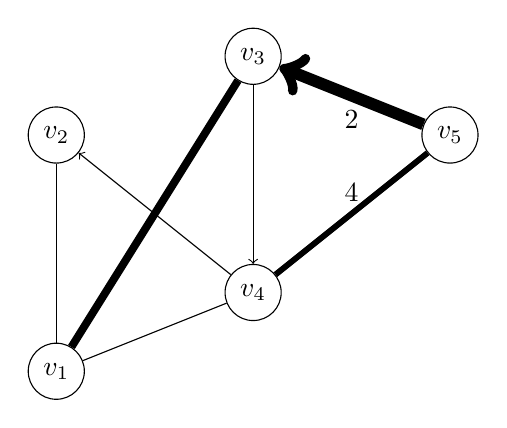
\begin{tikzpicture}
		% cette commande permet de créer un noeud, en précisant sa position spatiale (les valeurs entre parenthèses) et le texte qu'il contient (entre accolades). 
        %On peut également donner un nom interne au noeud (ici : A, B, C, D, etc.), qui sera utilisé plus tard par Tikz lors de la création des liens.
        \node[shape=circle,draw=black] (nnnn) at (0,0) {$v_1$};
		\node[shape=circle,draw=black] (node) at (0,3) {$v_2$};
		\node[shape=circle,draw=black] (truc) at (2.5,4) {$v_3$};
		\node[shape=circle,draw=black] (D) at (2.5,1) {$v_4$};
		\node[shape=circle,draw=black] (Zz) at (5,3) {$v_5$} ;
        
    	% cette commande ajoute un lien entre les noeuds dont les noms sont indiqués entre parenthèses
		\draw (nnnn) -- (node);
        \draw (nnnn) -- (D);
        % on peut changer l'épaisseur des liens de la façon suivante (pour les graphes pondérés)
		\draw[line width=1mm] (nnnn)  -- (truc);
        % toujours pour les graphes pondérés, on peut aussi rajouter des labels sur les liens (les positions optionnelles possibles sont left/right et above/below)
		\draw[line width=0.75mm] (D) -- (Zz) node [midway, left, above] {4};
		% on peut aussi orienter les liens de la façon suivante
        \draw[->] (truc) -- (D);
        % pour changer la taille de la flèche
        \draw[-{>[scale=1.5]}] (D) -- (node);
        % et on peut bien sûr combiner tout ça
        \draw[-{>[scale=2]}, line width=1.5mm] (Zz) -- (truc) node [midway, left, below] {2};
	% fin du diagramme
	\end{tikzpicture}
    \caption[Exemple de graphe]{Exemple de représentation d'un graphe, produite en utilisant la bibliothèque \texttt{TikZ}.}
	\label{fig:graphe}
\end{figure}

%%%
\paragraph{Diagramme.} Un diagramme TikZ s'insère dans un environnement \texttt{figure} (décrit en Section~\ref{sec:Figures}). Le code source ci-dessous correspond à la Figure~\ref{fig:graphe} :
\begin{lstlisting}[language={[LaTeX]TeX}, numbers=none]
\begin{figure}[htb]
	...
	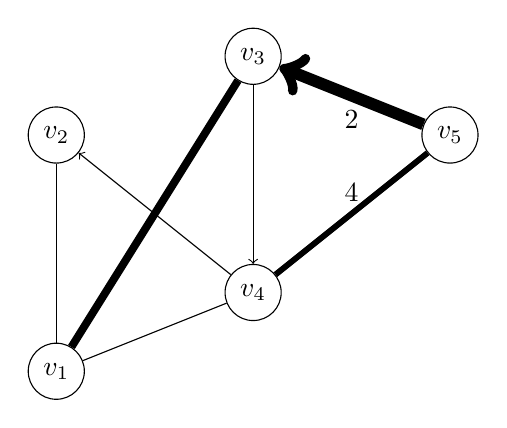
\begin{tikzpicture}
    	% sommets
		\node[shape=circle,draw=black] (nnnn) at (0,0) {$v_1$};
		\node[shape=circle,draw=black] (node) at (0,3) {$v_2$};
		\node[shape=circle,draw=black] (truc) at (2.5,4) {$v_3$};
		\node[shape=circle,draw=black] (D) at (2.5,1) {$v_4$};
		\node[shape=circle,draw=black] (Zz) at (5,3) {$v_5$} ;
        % liens
		\draw (nnnn) -- (node);	% une arête
		\draw (nnnn) -- (D);	% une autre arête
		\draw[line width=1mm] (nnnn)  -- (truc); % arête de poids différent
		\draw[line width=0.75mm] (D) -- (Zz) node [midway, left, above] {4};
		\draw[->] (truc) -- (D);	% arc
		\draw[-{>[scale=1.5]}] (D) -- (node); % arc avec une flèche plus grande
		\draw[-{>[scale=2]}, line width=1.5mm] (Zz) -- (truc) node [midway, left, below] {2};
	\end{tikzpicture}
    ...
\end{figure}
\end{lstlisting}

Le diagramme est défini au moyen de l'environnement \texttt{tikzpicture}. Les sommets sont insérés grâce à la commande \texttt{\textbackslash{}node[options] (nom) at (x,y) \{txt\};} (attention au point-virgule !), où :
\begin{itemize}
    \item \texttt{options} est une liste d'options graphiques, 
    \item \texttt{nom} est le nom interne du sommet (i.e. dans le cadre de TikZ, un nom utilisé plus tard pour définir les arêtes), 
    \item \texttt{(x,y)} est la position du sommet dans le plan, 
    \item \texttt{txt} est le texte affiché à l'intérieur du sommet.
\end{itemize}

Les arêtes sont insérées via de la commande \texttt{\textbackslash{}draw (s1) -\null- (s2);}, où \texttt{s1} et \texttt{s2} sont les \textit{noms internes} deux sommets connectés par l'arête. Pour une arête pondérée, on utilise l'option \texttt{line width} \texttt{\textbackslash{}draw}, qui permet de modifier l'épaisseur. Pour un arc, on utilise l'option \texttt{->} qui ajoute une flèche indiquant l'orientation de la relation.

%%%
\paragraph{Fichier externe.} Le script permettant de définir un graphe peut devenir assez vite long. Sa présence dans le code source du document y rend la navigation plus difficile. Pour éviter cela, il est possible d'externaliser ce code source, c'est à dire de le placer dans un fichier séparé, qui est ensuite importé dans le document principal.

On utilise pour cela la commande \texttt{\textbackslash{}input}, qui prend en paramètre le nom du fichier à inclure. Supposons qu'on déplace dans un fichier \texttt{diagrammes/graphe.tex} la partie du code source de la Figure~\ref{fig:graphe} correspondant à l'environnement \texttt{tikzpicture}. Alors, le code source dans le document principal peut être simplifié de la façon suivante :
\begin{lstlisting}[language={[LaTeX]TeX}, numbers=none]
\begin{figure}[htb]
	\centering
    \input{diagrammes/graphe.tex}
    \caption[Exemple de graphe]{Exemple de représentation d'un graphe, produite en utilisant la bibliothèque \texttt{TikZ}.}
	\label{fig:graphe}
\end{figure}
\end{lstlisting}
% \begin{figure}[htb]
% 	\centering
%     \input{diagrammes/graphe.tex}
%     \caption[Exemple de graphe]{Exemple de représentation d'un graphe, produite en utilisant la bibliothèque \texttt{TikZ}.}
% 	\label{fig:grapheExt}
% \end{figure}




%%%%%%%%%%%%%%%%%%%%%%%%%%%%%%%%%%%%%%%%%%%%%%%%%%%
\subsection{Diagrammes UML}
\label{sec:UML}
Pour les diagrammes UML, l'idéal est d'utiliser un outil externe spécialisé, pouvant produire soit un fichier contenant l'image sous forme de diagramme, soit directement du code \texttt{TikZ} à copier-coller dans le rapport. 

%%%
\paragraph{Fichier.} Comme cela a déjà été indiqué en Section~\ref{sec:Figures}, veillez à sélectionner un outil capable de produire des images \textit{vectorielles}~\cite{Wikipedia2018c}, par exemple au format PDF. Cela permet au lecteur de zoomer sans perte de qualité. Attention à ne pas enregistrer simplement une image \textit{matricielle}~\cite{Wikipedia2018b} dans un PDF : cela n'aurait aucun intérêt. 

De nombreux logiciels gratuits permettent d'éditer des diagrammes et de les enregistrer sous forme vectorielle. C'est notamment le cas du logiciel libre Dia \footnote{\url{http://dia-installer.de}}, qui est disponible pour la plupart des systèmes d'exploitation.

Une fois l'image exportée, son importation dans le rapport se fait exactement comme expliqué pour les images en Section~\ref{sec:Figures}.

%%%
\paragraph{Code source.}  Dia permet d'exporter les diagrammes au format PDF, mais il est aussi capable de générer directement du code \LaTeX{}, qui peut ensuite être intégré tel quel dans le document. Pour ce faire, suffit d'aller dans le menu \textit{Fichier} > \textit{Exporter}, et de choisir le format \textit{Macros PGF LaTeX (*.tex)}. 

\begin{figure}[htb!]
	\centering
	\resizebox{0.75\linewidth}{!}{\input{diagrammes/classdiag.tex}}
	\caption{Exemple de diagramme de classes.}
	\label{fig:diag}
\end{figure}

L'intérêt de cette approche, par rapport à un PDF, est de pouvoir modifier directement le code \LaTeX{} si on a des ajustement à apporter au diagramme. L'insertion de cette forme de diagramme dans le document se fait par l'environnement \texttt{figure}, en utilisant la commande \texttt{\textbackslash{}import} déjà introduite pour les graphes (Section~\ref{sec:Graphes}) : 
\begin{lstlisting}[language={[LaTeX]TeX}, numbers=none]
\begin{figure}[htb!]
	\centering
	\resizebox{0.75\linewidth}{!}{\input{diagrammes/classdiag.tex}}
	\caption{Exemple de diagramme de classes.}
	\label{fig:diag}
\end{figure}
\end{lstlisting}
Ce code source a pour résultat la Figure~\ref{fig:diag}, qui affiche le fichier \texttt{diagrammes/classdiag.tex} produit avec Dia. Notez que la commande \texttt{\textbackslash{}input} permet d'inclure du code \LaTeX{} situé dans un autre fichier, \textit{quel qu'il soit} (i.e. pas uniquement pour un diagramme comme ici). 

La commande \texttt{\textbackslash{}resizebox} permet simplement d'ajuster la taille du diagramme produit. Ici, la valeur $0.75$ indique que l'on utilise $75\%$ de la largeur correspondant à une ligne de texte.


%%%%%%%%%%%%%%%%%%%%%%%%%%%%%%%%%%%%%%%%%%%%%%%%%%%
\subsection{Diagrammes de Gantt}
\label{sec:Gantt}
Ce thème est configuré pour permettre l'insertion de diagrammes de Gant basiques tel que celui présenté dans la Figure~\ref{fig:gantt}, au moyen de la bibliothèque \texttt{pgfgantt}\footnote{\url{https://ctan.org/pkg/pgfgantt}}. Si vous trouvez mieux ailleurs, ou si vous avez besoin de plus de fonctionnalités, vous pouvez utiliser un autre outil, y compris externe. Cependant, veillez alors à ce que cet outil génère bien un fichier PDF. Notez que l'avantage de l'approche présentée ci-dessous est que le diagramme est facilement éditable directement dans le document \LaTeX{}.

\begin{figure}[htb!]
	\centering
   	\resizebox{0.95\linewidth}{!}{\input{diagrammes/ganttdiag.tex}}
    \caption{Diagramme de Gantt pour le premier semestre. Chaque couleur correspond à un étudiant : \textcolor{purple}{\textbf{Prénom1 Nom1}}, \textcolor{teal}{\textbf{Prénom2 Nom2}}, \textcolor{blue}{\textbf{Prénom3 Nom3}}, et \textcolor{orange}{\textbf{Prénom4 Nom4}}. Les $\sqdiamond$ représentent les séances de TP, tandis que les lignes verticales correspondent aux dates des rendus.}
	\label{fig:gantt}
\end{figure}

Pour définir un diagramme de Gantt, vous devez utiliser l'environnement \texttt{ganttchart}, lui même inséré dans un environnement \texttt{figure}. Il est possible de détailler les commandes décrivant le diagramme soit directement dans le document \LaTeX{} principal, soit dans un fichier \texttt{.tex} séparé qu'il faut alors importer avec la commande \texttt{\textbackslash{}input}, exactement comme nous l'avions fait pour les diagrammes UML en Section~\ref{sec:UML}. 

Dans le cas de l'exemple de la Figure~\ref{fig:gantt}, nous avons opté pour la seconde approche. L'extrait de code source ci-dessous présente les points principaux pour le diagramme contenu dans le fichier \texttt{diagrammes/ganttdiag.tex} :
\begin{lstlisting}[language={[LaTeX]TeX}, numbers=none]
\begin{figure}[htb!]
	...
    \setcounter{myWeekNum}{37} % semaine de départ
    \begin{ganttchart}[... 
            x unit=0.11cm,	% largeur d'une journée
			...,
        ]{2018-09-10}	% date de début de la période considérée
        {2019-01-20}	% date de fin de la période considérée
        % indications temporelles
    	\gantttitlecalendar[title/.style={fill=black!30,draw=black}]{year} \\
        ...
        % séances de TP
		\ganttmilestone{TP}{2018-09-13} %TP01
        ...
        % tâches
		\ganttbarbis{T01}{Tâche 01}{2018-10-03}{2018-10-29}{blue!50} \\
        ...
        % dates de rendu
		\drawverticalline{2018-09-16}{R1}
        ...
    \end{ganttchart}
    ...
\end{figure}
\end{lstlisting}

\begin{beware}[Remarque]
Bien entendu, il est recommandé d'externaliser le code source du diagramme de Gantt, grâce à la commande \texttt{\textbackslash{}input}, car ce code source est généralement assez long.
\end{beware}

%%%
\paragraph{Période représentée.} La commande \texttt{\textbackslash{}setcounter\{myWeekNum\}\{xx\}} permet d'indiquer le numéro \texttt{xx} (dans l'année) de la semaine de départ pour la période représentée.

Les deux derniers paramètres de l'environnement \texttt{ganttchart} doivent être utilisés pour indiquer le début et la fin de la période considérée. Dans l'exemple, il s'agit de \texttt{2018-09-10} et \texttt{2019-01-20}.

%%%
\paragraph{Jalons.} Il est possible de définir des jalons en utilisant la commande \texttt{\textbackslash{}ganttmilestone}. Elle prend en paramètre un texte optionnel (affiché dans la marge gauche du diagramme) et la date associée au jalon.

Ces jalons prennent la forme de losanges noirs dans le diagramme. Dans l'exemple, on les utilise pour représenter les séances de TP.

%%%
\paragraph{Tâches.} Les tâches sont ajoutées au moyen de la commande \texttt{\textbackslash{}ganttbarbis}, et prennent la forme de barres horizontales dans le diagramme. La commande prend en paramètre un nom court (affiché dans la marge gauche), un nom plus long (affiché dans la barre représentant la tâche) et une couleur (utilisée pour colorer la barre). Le nom long doit être ajusté pour tenir dans la largeur de la barre.

%%%
\paragraph{Échéances.} Les échéances apparaissent sous forme de droites verticales, obtenues au moyen de la commande \texttt{\textbackslash{}drawverticalline}. Celle-ci prend en paramètre une date permettant de situer l'échéance, et un nom court qui est placé au-dessous de la droite dans le diagramme.


%%%%%%%%%%%%%%%%%%%%%%%%%%%%%%%%%%%%%%%%%%%%%%%%%%%
\subsection{Figures géométriques}
\label{sec:Graphiques}
Il est possible de définir des figures géométriques manuellement grâce à \texttt{TikZ}, comme on l'a fait en Section~\ref{sec:Graphes} pour les graphes. Cependant il est plus pratique d'utiliser un éditeur WYSIWYM puis de l'exporter sous forme de fichier PDF ou de code \texttt{TikZ}. Nous en mentionnons deux ici (sans souci d'exhaustivité).

%%%
\paragraph{GeoGebra.} C'est ce que permet par exemple GeoGebra\footnote{\url{https://www.geogebra.org}}. Cet éditeur libre est disponible sous la forme d'une application bureau multiplateforme (à installer sur votre machine), mais aussi d'une application Web (avec des fonctionnalités réduites, néanmoins).

Il permet de composer le graphique ou la figure géométrique de façon intuitive. Il suffit ensuite d'aller dans son menu \textit{Download as} et de sélectionner \texttt{PDF} pour la télécharger sous forme de fichier PDF, ou bien \textit{PGF/TikZ} pour produire automatiquement un fichier contenant le code source \texttt{TikZ} correspondant. Vous pouvez ensuite insérer la figure dans le document \LaTeX{} à partir de l'image (PDF) avec \texttt{\textbackslash{}includegraphics}, ou à partir du code source avec \texttt{\textbackslash{}input}.

À titre d'exemple, la Figure~\ref{fig:geogebra} a été générée avec GeoGebra. Elle correspond aussi bien à l'image contenue dans le fichier \texttt{images/geogebra.pdf} qu'au code source du fichier \texttt{diagrammes/geogebra.tex}.

\begin{figure}[htb!]
	\centering
%	\resizebox{0.65\linewidth}{!}{\input{diagrammes/geogebra.tex}}
	\includegraphics[width=0.45\linewidth]{images/geogebra.pdf}
	\caption{Illustration de la démonstration du Théorème de Pythagore proposée par Euclide~\cite{Wikipedia2019}, générée au moyen de GeoGebra, et correspondant aux fichiers \texttt{diagrammes/geogebra.tex} et \texttt{images/geogebra.pdf}.}
	\label{fig:geogebra}
\end{figure}

%Attention cependant : il s'agit d'un document \LaTeX{} \textit{complet}, et non pas simplement du code \texttt{TikZ} correspondant à la figure elle-même. Il est donc nécessaire de nettoyer un peu ce fichier pour le débarrasser des instructions inutiles : \texttt{\textbackslash{}documentclass}, \texttt{\textbackslash{}usepackage}, \texttt{\textbackslash{}pgfplotsset}, \texttt{\textbackslash{}usetikzlibrary} \texttt{\textbackslash{}pagestyle}, \texttt{\textbackslash{}begin\{document\}} et \texttt{\textbackslash{}end\{document\}}. Il faut aussi déplacer les éventuelles couleurs définies par GeoGebra (\texttt{\textbackslash{}definecolor}) dans l'environnement \texttt{tikzpicture}. Référez-vous au fichier \texttt{diagrammes/geogebra.tex} pour visualiser le code source de la Figure~\ref{fig:geogebra}.

%%%
\paragraph{Alternatives.} On peut citer des alternative à GeoGebra, notamment l'application Web Matcha\footnote{\url{https://www.mathcha.io}}, qui fonctionne à peu près de la même manière, et l'application bureau multiplateforme et libre Inkscape\footnote{\url{https://inkscape.org}}, qui permet également de traiter des diagrammes plus généraux.








  
%%%%%%%%%%%%%%%%%%%%%%%%%%%%%%%%%%%%%%%%%%%%%%%%%%%
%% Code source
%%%%%%%%%%%%%%%%%%%%%%%%%%%%%%%%%%%%%%%%%%%%%%%%%%%
\section{Contenu à chasse fixe}
\label{sec:ChasseFixe}
Cette section est dédiée aux environnements permettant d'insérer du texte en utilisant une \textit{police à chasse fixe}~\cite{Wikipedia2018f} : code source (Section~\ref{sec:CodeSource}), contenu d'un fichier texte (Section~\ref{sec:ContenuFichier}), texte affiché dans une console (Section~\ref{sec:Console}). La plupart de ces fonctionnalités sont inutiles dans le cadre de cette UE, mais elles sont décrites par souci d'exhaustivité.



%%%%%%%%%%%%%%%%%%%%%%%%%%%%%%%%%%%%%%%%%%%%%%%%%%%
\subsection{Code source}
\label{sec:CodeSource}
Il est très déconseillé d'insérer du code source dans un rapport, car cela correspond à un niveau de détail qui est rarement nécessaire, et rallonge inutilement le document. Les éléments relatifs aux points de conception doivent plutôt être décrits en utilisant des diagrammes UML (Section~\ref{sec:UML}), tandis que ceux relatifs au traitement sont décrits de façon plus synthétique sous forme de pseudo-code (Section~\ref{sec:Algorithmes}). La présence de code source répond à un besoin vraiment très spécifique. Avant d'inclure du code source dans votre rapport, réfléchissez donc bien à la nécessité et à la pertinence de cette action. Dans le cadre de cette UE, n'incluez du code source que si cela vous est demandé explicitement.

Quoi qu'il en soit, ce thème permet d'insérer du code source grâce à la bibliothèque \texttt{listings}\footnote{\url{https://ctan.org/pkg/listings}} et à son environnement \texttt{lstlisting} : 
\begin{lstlisting}[language=Java]
// Hello.java
import javax.swing.JApplet;
import java.awt.Graphics;

public class Hello extends JApplet
{	public void paintComponent(Graphics g) 
	{	g.drawString("Hello, world!", 65, 95);
	}    
}
\end{lstlisting}

Le code source correspondant au listing précédent est le suivant :
\begin{TeXlstlisting}
\begin{lstlisting}[language=Java]
// Hello.java
import javax.swing.JApplet;
import java.awt.Graphics;

public class Hello extends JApplet
{	public void paintComponent(Graphics g) 
	{	g.drawString("Hello, 'world'!", 65, 95);
	}    
}
\end{lstlisting}
\end{TeXlstlisting}

%%%
\paragraph{Langage de programmation.} L'option \texttt{language} de l'environnement \texttt{lstlisting} permet de spécifier le langage du code source mentionné (ici : Java).

%%%
\paragraph{Positionnement.} Remarquez qu'à la différence du pseudocode (Section~\ref{sec:Algorithmes}), nous ne considérons pas le code source comme un élément flottant, et il n'est par conséquent pas numéroté. La raison en est que l'environnement \texttt{lstlisting} autorise que son contenu soit coupé par un changement de page quand cela est nécessaire. Par conséquent, \LaTeX{} le place toujours exactement là où il est défini dans le document, et n'a pas besoin de le déplacer ailleurs comme c'est parfois le cas pour les figures ou autres éléments flottants.

%%%
\paragraph{Légende.} Il est cependant possible d'avoir besoin de faire un renvoi vers du code source situé ailleurs dans le document. On a alors besoin de définir un numéro et un label pour ce listing. Ceci est possible grâce à aux options \texttt{caption} et \texttt{label} de l'environnement \texttt{lstlisting}, qui fonctionnent comme les commandes de même nom utilisées avec les éléments flottants. 

Par exemple, pour rajouter une légende au listing précédent, on fait :
\begin{TeXlstlisting}
\begin{lstlisting}[language=Java,caption={Applet Java affichant le message \textit{Hello World !}},label={lst:exemple}]
// Hello.java
import javax.swing.JApplet;
...
\end{lstlisting}
\end{TeXlstlisting}
Ce qui donne le résultat suivant :
\begin{lstlisting}[language=Java,caption={Applet Java affichant le message \textit{Hello World !}},label={lst:exemple}]
// Hello.java
import javax.swing.JApplet;
...
\end{lstlisting}
On peut faire référence à ce listing avec la commande \texttt{\textbackslash{}ref}, comme on le ferait avec un élément flottant : Listing~\ref{lst:exemple}.


%%%%%%%%%%%%%%%%%%%%%%%%%%%%%%%%%%%%%%%%%%%%%%%%%%%
\subsection{Contenu d'un fichier}
\label{sec:ContenuFichier}
Cette classe \LaTeX{} propose un environnement spécifique à l'affichage du contenu de fichiers texte. À l'instar du code source, l'utilisation de cet environnement ne sera pas fréquente pour cette UE.

L'environnement s'appelle \texttt{filetext}, et il est basé sur la bibliothèque \texttt{framed}\footnote{\url{https://ctan.org/pkg/framed}} :
\begin{filetext}
Première ligne du fichier texte ; \\
deuxième ligne, avec de la couleur \textcolor{red}{ici}, \hl{là}, et \colorbox{green}{là} ; \\
et enfin une troisième ligne.
\end{filetext}
Le code source correspondant est le suivant :
\begin{lstlisting}[language={[LaTeX]TeX}, numbers=none]
\begin{filetext}
Première ligne du fichier texte ; \\
deuxième ligne, avec de la couleur \textcolor{red}{ici}, \hl{là}, et \colorbox{green}{là} ; \\
et enfin une troisième ligne.
\end{filetext}
\end{lstlisting}

Notez que les retours à la ligne doivent être indiqués explicitement avec \texttt{\textbackslash{}\textbackslash{}}. Comme illustré dans l'exemple ci-dessus, il est possible de mettre certaines parties du contenu textuel en relief, modifiant la couleur du texte ou de l'arrière-plan.

%%%
\paragraph{Positionnement.} Comme pour le code source (Section~\ref{sec:CodeSource}), cet environnement n'est pas un élément flottant. Il n'est pas numéroté et apparaît là où il est défini. Au cas où on voudrait faire un renvoi vers ce type d'élément plus tard, il est toutefois possible de forcer la définition d'un titre et d'un numéro. On utilise pour cela les options \texttt{caption} et \texttt{label} de l'environnement, comme c'était déjà le cas pour \texttt{lstlisting} :
\begin{lstlisting}[language={[LaTeX]TeX}, numbers=none]
\begin{filetext}[caption={Contenu d'un fichier texte avec légende},label={fil:exemple}]
...
\end{filetext}
\end{lstlisting}
Ce code source produit le Fichier~\ref{fil:exemple}.
\begin{filetext}[caption={Contenu d'un fichier texte avec légende},label={fil:exemple}]
Contenu d'un fichier texte, cette fois avec une légende.
\end{filetext}





%%%%%%%%%%%%%%%%%%%%%%%%%%%%%%%%%%%%%%%%%%%%%%%%%%%
\subsection{Console}
\label{sec:Console}
Cette classe \LaTeX{} propose également un environnement dédié à l'affichage d'interactions avec une console système. À l'instar de l'environnement permettant d'afficher le contenu de fichiers textuels (Section~\ref{sec:ContenuFichier}), celui-ci est basé sur la bibliothèque \texttt{framed}, et son utilisation sera très rare dans le cadre de cette UE.

L'environnement se nomme \texttt{consoletext} et son rendu est le suivant :
\begin{consoletext}
invite/>macommande monparametre \& \\
macommande: command not found \\
invite/>$\blacksquare$
\end{consoletext}
Il fonctionne exactement comme l'environnement \texttt{filetext}, seul le rendu visuel est différent :
\begin{lstlisting}[language={[LaTeX]TeX}, numbers=none]
\begin{consoletext}
invite/>macommande monparametre \& \\
macommande: command not found \\
invite/>$\blacksquare$
\end{consoletext}
\end{lstlisting}

Il est là aussi possible de forcer l'insertion d'une légende et d'un numéro, comme pour les contenus de fichiers textes (Section~\ref{sec:ContenuFichier}), en procédant exactement de la même façon. Le rendu obtenu est illustré par la Console~\ref{con:exemple}.

\begin{consoletext}[caption={Invite de commande},label={con:exemple}]
invite/>$\blacksquare$
\end{consoletext}





  
%%%%%%%%%%%%%%%%%%%%%%%%%%%%%%%%%%%%%%%%%%%%%%%%%%%
%% Conclusion
%%%%%%%%%%%%%%%%%%%%%%%%%%%%%%%%%%%%%%%%%%%%%%%%%%%
\section{Conclusion}
\label{sec:Conclusion}
Il est recommandé de consulter le code source de ce document pour compléter les explications que vous venez de lire.

\LaTeX{} nécessite un minimum d'effort pour être pris en main, mais il n'y a rien d'insurmontable, notamment pour des étudiants en informatique (d'autant plus s'ils sont déjà familiers de langages comme HTML). Le contrôle obtenu et le rendu du document sont largement supérieurs à ceux des logiciels de traitement de texte, y compris commerciaux comme MS~Word. 

À noter qu'un très grand nombre d'extensions existent pour traiter des besoins spécifiques : diagrammes particuliers, documents de présentation de type Powerpoint, etc. Il est aussi possible d'intégrer du code Python ou R (ou autres langages) dans un document \LaTeX{}, qui sera réexécuté à chacune de ses compilations. À vous d'explorer toutes ces possibilités~!


 
 
  
  
  
  
  
  
%%%%%%%%%%%%%%%%%%%%%%%%%%%%%%%%%%%%%%%%%%%%%%%%%%%
%% Bibliographie
%%%%%%%%%%%%%%%%%%%%%%%%%%%%%%%%%%%%%%%%%%%%%%%%%%%
\MyBibliography


\end{document}
